\documentclass[runningheads]{llncs}
%% \documentclass[a4paper, anonymous, thm-restate]{lipics-v2021}
%%\documentclass[conference]{lipics}

% \IEEEoverridecommandlockouts
% The preceding line is only needed to identify funding in the first footnote. If that is unneeded, please comment it out.

%\usepackage{lmodern}
%\usepackage[nocompress]{cite}
\usepackage{hyperref}
%% url
\usepackage{url}
%% maths
\usepackage{amsmath,amssymb}
\usepackage{bm,centernot}
%% \usepackage{amsfonts}
%% \usepackage{amsthm}

%% algorithms
\usepackage{algorithmicx}
\usepackage[ruled, linesnumbered, noend]{algorithm2e}
\usepackage{multicol}

%% images
\usepackage{graphicx}
\usepackage[dvipsnames]{xcolor}
%% inparaenum
\usepackage{paralist}
%% TODO
% \usepackage{todonotes} %% after paralist to avoid clashes
% \newcommand{\note}[1]{\todo[size=\tiny]{#1}}
% \setlength{\marginparwidth}{2cm}
%% tables
\usepackage{booktabs, tabularx, multirow}
%% figures
%\usepackage{caption}
\usepackage{subfig}
\usepackage{tikz}
\usetikzlibrary{decorations.pathreplacing,plotmarks,shapes,matrix}
%% transform eps in pdf crossplateform
\usepackage{epstopdf}
\usepackage{epsfig}

\usepackage{xspace}
\usepackage{pifont}% http://ctan.org/pkg/pifont
\newcommand{\cmark}{\ding{51}}%
\newcommand{\xmark}{\ding{55}}%

\newcommand{\NAME}[0]{\mbox{AS-cast}\xspace}
\newcommand{\NAMEB}[0]{\mbox{S-cast}\xspace}
\newcommand{\NAMEC}[0]{\mbox{xAS-cast}\xspace}
\newcommand{\TODO}[1]{\textcolor{red}{#1}}
\newcommand{\REF}[0]{\textcolor{purple}{REF}\xspace}

\newcommand{\PA}[0]{RoyalBlue} %% used to be skyblue
\newcommand{\PB}[0]{BurntOrange}
\newcommand{\PC}[0]{Green}
\newcommand{\PD}[0]{\PC}
\newcommand{\WRONG}[0]{red!75}

% \newtheorem{problem}{Problem Statement}
% \newtheorem{definition}{Definition}
%% \newtheorem{lemma}{Lemma}
% \newtheorem{theorem}{Theorem}
% \newtheorem{corollary}{Corollary}
\newcommand{\eventually}{\Diamond\,}
\newcommand{\ie}{{i.e.,}\xspace}
\newcommand{\eg}{{e.g.,}\xspace}

\newcommand{\process}{node\xspace}
\newcommand{\processes}{nodes\xspace}
\newcommand{\Process}{Node\xspace}
\newcommand{\Processes}{Nodes\xspace}
\newcommand{\node}{\process}
\newcommand{\nodes}{\processes}
\newcommand{\Node}{\Process}
\newcommand{\Nodes}{\Processes}

\title{\NAME: Lock Down the Traffic\\of Decentralized Content Indexing at the Edge}
% \titlerunning{\NAME: Lock Down the Traffic of Decentralized Content Indexing at the Edge}

%% \keywords{
%%   Edge, decentralized content indexing, scoped
%%   broadcast, logical partitioning
%% }

%% \ccsdesc[500]{Networks~Network protocols}

%% \author{\IEEEauthorblockN{Adrien L{\`e}bre, Brice N{\'e}delec, Alexandre Van Kempen}
%%   \IEEEauthorblockA{\textit{Inria / LS2N}, Nantes, France\\first.last@inria.fr}
%% }

% \author{Anonymous}
%% \author{\IEEEauthorblockN{Adrien L{\`e}bre}
%%   \IEEEauthorblockA{\textit{Inria / LS2N}, Nantes, France\\adrien.lebre@inria.fr}
%%   \and
%%   \IEEEauthorblockN{Brice N{\'e}delec}
%%   \IEEEauthorblockA{\textit{LS2N}, Nantes, France\\brice.nedelec@ls2n.fr}
%%   \and
%%   \IEEEauthorblockN{Alexandre Van Kempen}
%%   \IEEEauthorblockA{\textit{Qarnot computing}, Montrouge, France\\alexandre.vankempen@qarnot-computing.com}
%% }

\begin{document}

% \proceedings{}
%\copyright{Adrien l{\'ebre}, Brice N{\'e}delec, Alexandre Van Kempen}

\maketitle


\begin{abstract}

  Fog infrastructures allows content providers to better distribute
  data over autonomous systems, hence improving on quality of user
  experience by reducing latency. However, locating the closest data
  sources can prove challenging in dynamic networks with dynamic
  sources. Locating sources may effectively take more time than
  actually downloading contents. \TODO{Related work ?} In this paper,
  we introduce \NAME, a reactive protocol for dynamic logical
  partitioning in dynamic networks. \TODO{source automatically create
    partitions.} \NAME uses epidemic dissemination (\TODO{scoped
    flooding}). \TODO{costs of operations.} When the system becomes
  quiescent, every process eventually converges to its closest
  partition, then \NAME incurs no overhead. \TODO{Proof, simulation,
    testbed?}

\end{abstract}


%%% Local Variables: 
%%% mode: latex
%%% TeX-master: "../paper"
%%% ispell-local-dictionary: "english"
%%% End: 



\section{Introduction}


\begin{figure*}
\centering
\subfloat[Initial configuration - Every nodes get the content from node $R$\label{fig:partition_intuitionA}]{\includegraphics[trim=6cm 0.33cm 6cm 0.33cm, clip, width=0.24\textwidth]{img/Dynamic-partitioning-1.png}}\hfill
\subfloat[Adding a second replica in node $G$ partitions the network nodes in $2$ sets.\label{fig:partition_intuitionB}]{\includegraphics[trim=6cm 0.33cm 6cm 0.33cm, clip, width=0.24\textwidth]{img/Dynamic-partitioning-2.png}}\hfill
\subfloat[A third replica is created in node $B$ resulting in $3$ partitions.\label{fig:partition_intuitionC}]{\includegraphics[trim=6cm 0.33cm 6cm 0.33cm, clip, width=0.24\textwidth]{img/Dynamic-partitioning-3.png}}\hfill
\subfloat[Removing the green partition: only $2$ partitions remain.\label{fig:partition_intuitionD}]{\includegraphics[trim=6cm 0.33cm 6cm 0.33cm, clip, width=0.24\textwidth]{img/Dynamic-partitioning-4.png}}
%
\caption{Example of the french RENATER topology (edges are not drawn):
  Partitions shrink or expand according to the creation or removal of
  replicas. Ideally, only a subset of nodes should be informed of
  these events, according to their place in the
  topology.} \label{fig:partition_intuition}
\end{figure*}

%%% Local Variables: 
%%% mode: latex
%%% TeX-master: "../paper"
%%% ispell-local-dictionary: "english"
%%% End: 
 %% positioning

In recent years, the data storage paradigm shifted from centralized in
the cloud to distributed at the edges of the network. 
% There is an ongoing evolution of storing data from the cloud to the
% edges of the network.
This shift aims at keeping the data close to
\begin{inparaenum}[(i)]
\item its producers since data may be too expensive or sensitive to be
  transmitted through the network; and
\item its consumers so data may quickly and efficiently reach
  them~\cite{cachier, foggy_cache, shi2016edge}.
\end{inparaenum}
%% It avoids transmitting Either because it is where it has been
%% created and it is too expensive to be transmitted through the
%% network, or because it has been replicated to bring data closer to
%% the end users ~\cite{shi2016edge, foggy_cache, cachier}.
%
To favour this transition, new designs for data management across Edge
infrastructures have been investigated~\cite{confais2017object,
  confais2017performance, fogstore, hasenburg2020towards}.  They
enable strategies to confine traffic by writing data locally and
replicating content according to effective needs. However, locating
content remains challenging. Retrieving a content location may
actually take more time than retrieving the content itself.
%% Although
%% these systems, provide good properties such as favouring network
%% traffic confinement by writting data locally and replicating contents
%% according to the effective needs, determining the location where to
%% get the content might be more expensive than retrieving the content
%% itself.
%
Indeed, these systems, when not using a centralized index hosted in a
Cloud~\REF, rely on distributed hash
tables~\cite{maymounkov2002kademlia} spread across the different
\processes composing the infrastructure. When a client wants to access
specific content, it requests a remote \process to provide at least
one \process identity to retrieve this content from. After it
retrieved the content, the client can create another replica to
improve the performance of future accesses, but it must contact the
content indexing service again to notify of such change.
%% a local replica is created to improve the performance for future
%% accesses and the process in charge of maintaining the index is
%% contacted once again to reflect this new location.
%

%This strategy has two majors drawbacks :
%\begin{itemize}
%  \item (i) the lookup penalty: the network latency to reach this
%    remote node incurs an additional delay~\cite{asrese2019measuring,
%      doan2019tracing} to get the object before
%    being able to start its downloading ;
%  \item (ii) the selection of the node(s) from which the content is
%    returned: due to the lack of information that would allow the  a request to each process storing a
%%    replica is perfomed in
%\end{itemize}

These approaches directly contradict with the objectives of Edge
infrastructures that aim at reducing the impact of latency as well as
the volume of data passing through the network.
%
First, accessing a remote \node to request content location(s) raises
hot spots and availability issues. But most importantly, it results in
additional delays that occur even before the actual download
started~\cite{asrese2019measuring, doan2019tracing}.
%
Second, the client gets a list of content locations at the discretion
of content indexing services. Without information about these
locations, it often ends up downloading from multiple replica hosts,
yet only keeping the fastest answer~\REF. In turns, either clients
waste network resources, or face lower response time. 
%% there is no information to select the ``best'' node among the
%% possible candidates from which the content could be retrieved. In
%% most cases, this results in parallel requests performed by the
%% client node to each candidate with the goal of retrieving the
%% content as efficient as possible.

To tackle aforementioned limitations, every \process that might
request or replicate content must also host its own content indexing
service in a fully decentralized fashion~\cite{kermarrec2015want}. At
any time, it can immediately locate the closest replica of specific
content.  A naive approach would be that every \process indexes and
ranks \emph{every live} replica along with its \emph{location}
information. When creating or destroying a replica, a \process would
notify all other \processes by efficiently broadcasting its
operation~\cite{birman1999bimodal, hadzilacos1994modular,
  raynal2013distributed}. Unfortunately, this also contradicts with
Edge infrastructure objectives, for such protocol does not confine the
traffic generated to maintain its indexes. A \process may acknowledge
the existence of replicas at the other side of the network while there
already exists a replica right next to it.

Instead, a \process creating a replica should notify all and only
\processes that have no closer replica. This would create
interconnected sets of \processes, or \emph{partitions}, gathered
around a \emph{source} being their respective replica. A \process
deleting its replica should notify all members of its partition so
they can rally their current closest partition. A periodic
advertisement protocol already provides both these operations for
routing purposes~\cite{hemmati2015namebased}. However, its functioning
requires
\begin{inparaenum}[(i)]
\item to generate traffic even when the system is quiescent, and
\item to finely tune physical-time-based intervals that depend on
  network topology parameters such as network diameter.
\end{inparaenum}

%% A ``simple'' way to tackle the aforementioned limitations would be to
%% maintain on each node composing the infrastructure and for each
%% content, an index of all replicas (and their ``distance'').  In such
%% an approach, each time a new replica is created or deleted, a message
%% is broadcasted from the node that performed the operation (\ie the
%% source) to all nodes, increasing the distance information at each hop.
%% %
%% In addition to being complicated for large-scale systems, maintaining
%% a global view on each node is useless as there is no interest to
%% inform a node of the creation/removal of a replica at the opposite of
%% the network (each node trying to get content from the ``closest''
%% one).  In other words, the broadcast should be limited to a partition
%% of the infrastructure, (\ie the subset of nodes that has to update the
%% current location for this particular content). Obviously, these
%% partitions depend and evolve according to concurrent operations made
%% by nodes (replica creation/removal) as well as dynamic changes in the
%% infrastructure (network failures, node apparitions/leaves).

In this paper, we propose a first implementation of such a protocol.
Entitled Adaptive Scoped broadcast (\NAME), 
our protocol relies on a primitive that forwards
messages until a certain condition is reached, \ie the scope. The
scope is defined by a boolean function (predicate) that returns
whether a message should be propagated or not around its
broadcaster. In the current scenario, the stop condition is related to
the distance to the nearest replica : if the message that a node receives
indicates a content has a longer distance than that which the node
knows then the transfer of the message is useless and so stopped.
%
This primitive is used to guarantee that eventually, every node knows
its best partition, hence its closest replica, despite concurrent
events and receipt orders. Overall, \NAME is a wait-free reactive protocol for
dynamic logical partitioning.  Its overhead actually depends on
its operations and current partitions in the system. When the system
becomes quiescent, nodes eventually converge to their respective
partition and do not require further communication afterward.

\TODO{talk about the proof}

We evaluated our protocol through two simulation scenarios using
\textit{Peersim}~\cite{montresor2009peersim}. First, we confirm that
\NAME allow consistent partitioning in an ad-hoc network composed of
10K nodes.  Second, we illustrate how \NAME enables the lock down of
the traffic in dynamic inter autonomous systems.  More precisely, we
simulated a worldwilde infrastructure by duplicating the GEANT
topology - a real infrastructure spanning across Europe – and by
connecting these two clusters with a high latency link: 200 ms
simulating cross-continental communications such as Europe-America.

%
\begin{figure*}
  \begin{center}
    \subfloat[Part A][\label{fig:addA}Both Process $a$ and
      Process $c$ initiate a partition.
      $w_{ab} = 1.5$; $w_{bc} = w_{cd} = w_{bd} = 1$.]{
\begin{tikzpicture}[scale=1]

  \newcommand\X{50pt}
  \newcommand\Y{-50pt}


  \draw[fill=white] (0, 0) node{$\bm{a}$} +(-5, -5) rectangle +(5, 5);
  


\end{tikzpicture}
}
    \hspace{5pt}
    \subfloat[Part B][\label{fig:addB}Messages transit through communication
      links and carry increasing weights.]{
\begin{tikzpicture}[scale=\SCALE]

  \draw (-\X + 5pt, 0) --
  node[above=-0.3em, left=-0.3em, above left, font=\SMSG]{$\textcolor{\PA}{\alpha_a^2} \RIGHT$}
  (0 - 5pt, 0); %% b - a 

  \draw (0 +5pt, 0) --
  (\X -5pt, 0); %% c - b

  \draw[opacity=0] (0, 0 - 5pt) --
  % node[opacity=1, above=-0.3em, font=\tiny, sloped]{$\textcolor{\PA}{\ADD_a^{3}} \RIGHT$}
  (0, \Y + 5pt); %% b - d
  \draw (0, \Y + 5pt) --
  node[above=-0.3em, font=\SMSG, sloped]{$\textcolor{\PD}{\alpha_d^1} \RIGHT$}
  (0, 0 - 5pt);  %% d - b
  
  \draw (\X + 3pt, 0 - 5pt) --
  node[above=-0.3em, sloped, font=\SMSG]{$\textcolor{\PD}{\alpha_{d}^{3}} \RIGHT$}
  (0 + 5pt, \Y - 3pt); %% c - d



  \draw[fill=white] (-\X, 0)
  node[color=\PA]{$\bm{a}$}
  +(-5pt, -5pt) rectangle +(5pt, 5pt);  
  \draw[fill=white] (0, 0) node{$\bm{b}$} +(-5pt, -5pt) rectangle +(5pt, 5pt);
  \draw[fill=white] (\X, 0) node{$\bm{c}$} +(-5pt, -5pt) rectangle +(5pt, 5pt);
  \draw[fill=white] (0, \Y) node[color=\PD]{$\bm{d}$} +(-5pt, -5pt) rectangle +(5pt, 5pt);
  
  \draw (-\X, 5pt) node[above, font=\small, color=\PA]{$\alpha_a^0$};
  \draw (-5pt, \Y) node[left, font=\small, color=\PD]{$\alpha_d^0$};

\end{tikzpicture}
}
    \hspace{5pt}
    \subfloat[Part C][\label{fig:addC}Process $b$ receives and forwards
      $\alpha_{c}^{1}$ then discards $\alpha_{a}^{1.5}$, for the latter distance
      is higher.]{
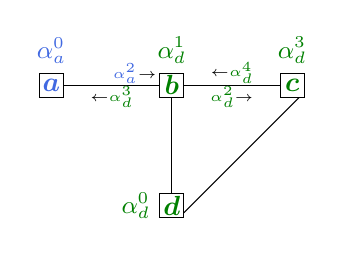
\begin{tikzpicture}[scale=0.87]

  \thickmuskip=0mu
  \medmuskip=0mu
  \thinmuskip=0mu
  
  \newcommand\X{50pt}
  \newcommand\Y{-50pt}

  \newcommand\ADD{\alpha}


  
  \draw (-\X + 5pt, 0) --
  node[above=-0.3em, right=-0.3em, above right, font=\tiny]{$\textcolor{\PA}{\ADD_a^2} \rightarrow$}
  node[below=-0.3em, font=\tiny]{$\leftarrow \textcolor{\PD}{\ADD_d^3}$}
  (0 - 5pt, 0); %% b - a 

  \draw (0 +5pt, 0) --
  node[above=-0.3em, font=\tiny]{$\leftarrow \textcolor{\PD}{\ADD_d^4}$}  
  node[below=-0.3em, font=\tiny]{$\textcolor{\PD}{\ADD_d^2} \rightarrow$}  
  (\X -5pt, 0); %% b - c

  \draw[opacity=0] (0, 0 - 5pt) --
  % node[opacity=1, above=-0.3em, font=\tiny, sloped]{$\ADD_{c}^{2} \rightarrow$}
  (0, \Y + 5pt); %% b - d
  \draw (0, \Y + 5pt) --
  % node[above=-0.3em, font=\tiny, sloped]{$\ADD_{c}^{2} \rightarrow$}
  (0, 0 - 5pt);  %% d - b
  
  \draw (\X + 3pt, 0 - 5pt) --
  % node[above=-0.3em, sloped, font=\tiny]{$\ADD_{c}^{2} \rightarrow$}
  (0 + 5pt, \Y - 3pt); %% c - d


  
  \draw[fill=white] (-\X, 0)
  node[color=\PA]{$\bm{a}$}
  +(-5pt, -5pt) rectangle +(5pt, 5pt);  
  \draw[fill=white] (0, 0)
  node[color=\PC]{$\bm{b}$}
  +(-5pt, -5pt) rectangle +(5pt, 5pt);
  \draw[fill=white] (\X, 0)
  node[color=\PC]{$\bm{c}$}
  +(-5pt, -5pt) rectangle +(5pt, 5pt);
  \draw[fill=white] (0, \Y)
  node[color=\PC]{$\bm{d}$}
  +(-5pt, -5pt) rectangle +(5pt, 5pt);

  \draw ( 0, 5pt) node[above, font=\small, color=\PD]{$\ADD_d^1$}; % b
  \draw ( \X, 5pt) node[above, font=\small, color=\PD]{$\ADD_d^3$}; % c
  \draw (-\X, 5pt) node[above, font=\small, color=\PA]{$\ADD_a^0$}; % a
  \draw (-5pt, \Y) node[left, font=\small, color=\PD]{$\ADD_d^0$}; % d
  
\end{tikzpicture}
}
    \hspace{5pt}
    \subfloat[Part D][\label{fig:addD}Processes $b$, $c$, and $d$ discard
      incoming messages. The system converged to optimal partitions.]{
      
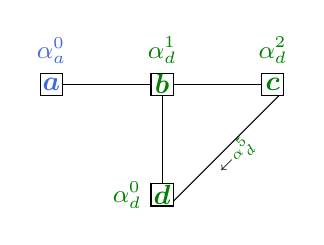
\begin{tikzpicture}[scale=0.8]

  \thickmuskip=0mu
  \medmuskip=0mu
  \thinmuskip=0mu
  
  \newcommand\X{50pt}
  \newcommand\Y{-50pt}

  \newcommand\ADD{\alpha}


  
  \draw (-\X + 5pt, 0) -- (0 - 5pt, 0); %% a - b

  \draw (0 +5pt, 0) --
  (\X -5pt, 0); %% b - c

  \draw (0, \Y + 5pt) --
  (0, 0 - 5pt);  %% d - b
  
  \draw (\X + 3pt, 0 - 5pt) --
  node[below=-0.3em, sloped, font=\tiny]{$\leftarrow \textcolor{\PD}{\ADD_{d}^{5}}$}
  (0 + 5pt, \Y - 3pt); %% c - d


  
  \draw[fill=white] (-\X, 0)
  node[color=\PA]{$\bm{a}$}
  +(-5pt, -5pt) rectangle +(5pt, 5pt);  
  \draw[fill=white] (0, 0)
  node[color=\PC]{$\bm{b}$}
  +(-5pt, -5pt) rectangle +(5pt, 5pt);
  \draw[fill=white] (\X, 0)
  node[color=\PC]{$\bm{c}$}
  +(-5pt, -5pt) rectangle +(5pt, 5pt);
  \draw[fill=white] (0, \Y)
  node[color=\PC]{$\bm{d}$}
  +(-5pt, -5pt) rectangle +(5pt, 5pt);
  
  \draw ( 0, 5pt) node[above, font=\small, color=\PD]{$\ADD_d^1$}; % b
  \draw ( \X, 5pt) node[above, font=\small, color=\PD]{$\ADD_d^2$}; % c
  \draw (-\X, 5pt) node[above, font=\small, color=\PA]{$\ADD_a^0$}; % a
  \draw (-5pt, \Y) node[left, font=\small, color=\PD]{$\ADD_d^0$}; % d

  
\end{tikzpicture}
}
    \caption{\label{fig:add}Simple accumulation in messages makes the
      system converge to consistent partitioning with scoped
      broadcast.}
  \end{center}
\end{figure*}

%%% Local Variables: 
%%% mode: latex
%%% TeX-master: "../paper"
%%% ispell-local-dictionary: "english"
%%% End: 

 %% positioning (belong to problem & motivation)

The rest of this paper is organized as
follows. Section~\ref{sec:background} introduces background, and
details the motivation behind our proposal.
Section~\ref{sec:adaptive} describes the protocol behavior, as well
as the formal definition of the underlying
algorithms. Section~\ref{sec:experimentation} presents the Peersim
evaluations.  Related work is discussed in
Section~\ref{sec:related_work} and finally
Section~\ref{sec:conclusion} concludes this article and highlights a
few future works.
  

%%% Local Variables: 
%%% mode: latex
%%% TeX-master: "../paper"
%%% ispell-local-dictionary: "english"
%%% End: 


\section{Background and motivation}
\label{sec:background}

\TODO{More related work. More motivations etc. Maybe describe IPFS?}

%% \begin{definition}[Dynamic optimal partitioning]
%%   A dynamic optimal partitioning is an optimal partitioning where the
%%   set of sources $S$ does not monotonically increase. We suffix this
%%   set with \underline{t}ime $t$ : $S(t)$.  Process $i$ joins the set
%%   of sources by \underline{a}dding its partition with messages
%%   $\alpha_i^{0}$: $Add(i \not\in S(t)) \implies i \in S(t+1)$; and
%%   leaves the set of sources by \underline{d}eleting its partition with
%%   messages $\delta_i$: $Del(i \in S(t)) \implies i \not\in S(t+1)$.
%% \end{definition}

%% Unfortunately, due to differences in receipt order of messages between
%% processes, stale information may stop prematurely the propagation of
%% relevant messages leading to inconsistent partitioning.
%% \TODO{Figure~\ref{fig:del} shows that.}

One could solve this issue by using a conflict-free replicated data
type (CRDT) for set data structures~\cite{shapiro2011crdts}. CRDTs
require eventual delivery of messages to ensure convergence. All
processes need to receive, deliver, hence broadcast all
operations. Some processes may receive operations unnecessary to their
correct functioning, for these operations did not happen in their
locality.  One could also solve this issue by removing partitions that
were not advertised for a defined
time~\cite{hemmati2015namebased}. \TODO{check distance-vector
  protocols.} However, relying on physical timeout could lead to
either premature removals of partitions when they are still operating;
or slow convergence where processes believe they belong to a partition
that was removed (\TODO{plot ?}). In addition, since timeouts imply a
continuous maintenance of partitions, such partitioning protocol
incurs an overhead even in quiet contexts without dynamic partitions.

%% \begin{problem}[\label{prob:intra}Consistent partitioning]
%%   How to enable \emph{consistent} dynamic optimal partitioning in
%%   dynamic network using scoped flooding?
%% \end{problem}

% \TODO{Dynamic Multiple-sources All-destinations shortest path on
%  dynamic graphs?}

%% \begin{figure}
%%   \begin{center}
%%     \input{input/figASmotivation.tex}
%%     \caption{\label{fig:ASmotivation}Scoped flooding extended to
%%       objects, processes do not know about all partitions that exist
%%       in the whole distributed system.}
%%   \end{center}
%% \end{figure}

%% To further improve scoped flooding in autonomous systems, processes
%% may belong to multiple partitions representing the objects they are
%% aware of. Figure~\ref{fig:ASmotivation} highlights the geo-distributed
%% nature of autonomous systems. Autonomous systems have topological
%% properties~\cite{nur2018geography} that processes can leverage to
%% avoid flooding the whole systems with control information about all
%% partitions. In Figure~\ref{fig:ASmotivation}, Process $e$ creates a
%% partition about a specific object, flooding Paris's AS to notify
%% neighboring processes of the object. However, it does not flood the
%% whole network, for control information stops at Process $b$. It
%% significantly saves bandwidth compared to broadcast since processes
%% below entrypoints of autonomous systems are order of magnitude more
%% numerous. Yet, Processes $c$ and $d$ know whom to ask when they need
%% to return an object they are unaware of. Processes remain efficient in
%% answering requests. \TODO{which is important for end users \REF.}

%% \begin{definition}[Partitions in asynchronous systems]
%%   Processes may hold multiple partitions \TODO{Use $\mathcal{P}$}
%%   \TODO{TODO} \TODO{or multi-partitioning?}
%% \end{definition}

%% \begin{problem}[\label{prob:inter}Inter-AS consistent partitioning]
%%   How to enable scoped flooding of objects in autonomous systems?
%% \end{problem}

%% Next Section presents our approach that solves these scientific
%% problems by relying on logical control information only.

%%% Local Variables: 
%%% mode: latex
%%% TeX-master: "../paper"
%%% ispell-local-dictionary: "english"
%%% End: 



\section{Adaptive scoped broadcast}
\label{sec:adaptive}

To assign and maintain \processes to their best partition according to
replica creations and removals, as well as dynamic infrastructure
changes, we designed and implemented \NAME.  \NAME stands for
\underline{A}daptive \underline{S}coped broad\underline{cast}. It
relies on a primitive that allows a \process to broadcast a message
within a limited scope. We first use this primitive to guarantee
consistent partitioning when a \process can only create a new replica
within the system. We highlight the issue when a \process can also
destroy a replica, and provide a second algorithm that handles replica
removals as well as dynamic changes of the infrastructure.  This
section describes the communication primitive called scoped broadcast,
then discusses the properties that guarantee consistent partitioning,
and finally details our implementation \NAME.
% and the analysis of its complexity.


\subsection{Scoped broadcast}
\label{subsec:scoped}

%For instance, a \process from Paris could scoped broadcast messages to
%all \processes in Paris; and \processes from other cities would never
%deliver such messages.
%Scoped broadcast only targets a connected \emph{subset} of \processes
%in the whole distributed system.
%

% \TODO{dynamic graph: superscript with $t$?}
In this paper, we consider Edge infrastructures with heterogeneous
\nodes interconnected by communication links. \Processes involved in
the management of content may crash but are not byzantine.  \Processes
can reliably communicate through asynchronous message passing to other
known \processes called neighbors.  % A more formal
%definition of our system is given below:
We define scoped broadcast as a communication primitive that
propagates a message around its broadcaster within an
application-dependant scope.

\begin{definition}[Edge infrastructure]
  An Edge infrastructure is a connected \underline{g}raph $G(V, E)$ of
  \underline{v}ertices $V$ and bidirectional \underline{e}dges $E
  \subseteq V \times V$.  A \underline{p}ath $\pi_{ij}$ from
  \Process~$i$ to \Process~$j$ is a sequence of vertices $[i, k_1,
    k_2, \ldots k_n, j]$ with $\forall m: 0\leq m \leq n, \langle
  \pi_{ij}[m], \pi_{ij}[m+1] \rangle \in E$.
\end{definition}


%Using epidemic
%propagation (or gossiping), \processes can reliably broadcast messages
%by forwarding delivered messages from neighbors to
%neighbors~\cite{birman1999bimodal, hadzilacos1994modular,
%  nedelec2018causal, raynal2013distributed}.
%
%However, uniform reliable
%broadcast states that \emph{all} correct \processes must deliver all
%broadcast messages. This proves costly in large scale systems
%comprising thousands of \processes. Instead, we define \emph{scoped
%broadcast} where messages reach only an application-dependant subset
%of connected \processes, thus significantly reducing the generated
%traffic of broadcast.


\begin{definition}[\label{def:scoped}\underline{S}coped broad\underline{cast} (\NAMEB)]
  When \Process~$x$ scoped \underline{b}roadcasts $b_x(m)$ a
  \underline{m}essage $m$, every correct \process $y$ within a scope
  \underline{r}eceives $r_y(m)$ and \underline{d}elivers it
  $d_y(m)$. The scope depends on the \underline{s}tate $\sigma$ of
  each \process, the \underline{m}etadata $\mu$ piggybacked by each
  message, and a \underline{p}redicate $\phi$ verified from \process to
  \process: $b_x(m) \wedge r_y(m) \implies \exists \pi_{xy}: \forall z
  \in \pi_{xy}, \phi(\mu_z, \sigma_z)$.
\end{definition}

This definition encompasses more specific definitions of related
work~\cite{hsiao2005scoped, lue2006scoped, wang2015prodiluvian}.  It
also highlights that epidemic propagation and scoped broadcast have
well-aligned preoccupations. More precisely, it underlines the
transitive relevance of messages, thus a \process can stop forwarding
messages as soon as its predicate becomes unverified.
%For instance, a \process
%from Paris could scoped broadcast messages to all \processes in
%Paris. This requires \processes to store and maintain their city
%location in their local state. \Processes stop delivering and
%forwarding their received messages when they come from a different
%city.  In another instance, a \process from Paris could scoped
%broadcast messages to all \processes in Paris plus neighboring
%cities. This requires \processes to overload forwarded messages the
%first time they reach another city. The predicate checks if messages
%already reached two distinct cities before delivery. Similarly to
%uniform reliable broadcast, scoped broadcast implementations expose
%different trade-offs on space, time, and communication.
%
We use \NAMEB to efficiently modify the state of each \process
depending on the partitions that exist in the system.



\subsection{Consistent partitioning}
\label{subsec:consistent}

At any time, a \process can decide to become a \emph{source}, hence
creating a new partition in the system by executing an \texttt{Add}
operation. This partition includes at least its source plus
neighboring \processes that estimate they are closer to this source
than any other one. Such a distance (or \emph{weight}) is
application-dependant: in the context of maintaining distributed
indexes, this would be about link latency that \nodes could monitor
by aggregating \texttt{ping}s.

\begin{definition}[\label{def:partitioning}Partitioning]
  Let $S \subseteq V$ be the set of \underline{s}ources, and $P_s$ be
  the \underline{p}artition including at least \Process~$s$, each
  \process belongs to at most one partition $\forall p,q \in V, \forall
  s_1,s_2 \in S: p \in P_{s_1} \wedge q \in P_{s_2} \implies p \neq q
  \vee s_1 = s_2$, and there exists at least one path $\pi_{ps}$ of
  \processes that belong to this partition $\forall q \in \pi_{ps}: q
  \in P_s$.
\end{definition}

Definition~\ref{def:scoped} and Definition~\ref{def:partitioning}
share the transitive relevance of \process states. However, we further
constrain the partitioning in order to guarantee the existence of
exactly one consistent partitioning that \processes eventually converge
to.

\begin{definition}[\underline{C}onsistent \underline{p}artitioning (CP)]
  Let $W_{xy} = W_{yx}$ be the positive symmetric \underline{w}eight
  between $x$ and $y$, $\Pi_{xz}$ be the shortest \underline{p}ath
  from $x$ to $z$ the weight of which $|\Pi_{xz}|$ is lower than any
  other path weight, with $|\Pi_{xx}|$ being the greatest lower bound
  of $x$, the only consistent partitioning $\mathcal{P}$ is a set of
  partitions $P_{s\in S}$ such that each \process belongs to a logical
  partition comprising its closest source: $\forall p \in P_{s_1}:
  \nexists P_{s_2}$ such that $|\Pi_{s_2p}| < |\Pi_{s_1p}|$.
\end{definition}

Unfortunately, \processes do not share a common global knowledge of
the network state. For \processes to reach consistent partitioning
together, a \Process $s$ \underline{a}dding a partition must send a
notification $\alpha_s$ to every \process that is closer to it than
any other source. Since epidemic dissemination and scoped broadcast
have well-aligned preoccupations, we assume implementations relying on
message forwarding from neighbor-to-neighbor.

\begin{theorem}[\label{theo:efb}\underline{E}ventual \underline{F}orwarding
    of \underline{B}est $(EFB) \implies CP$] Assuming reliable
  communication links where a correct \process $q$ eventually receives
  the message $m$ \underline{s}ent to it by a \process $p$ ($s_{pq}(m)
  \implies r_{q}(m)$), \processes eventually reach consistent
  partitioning if each \process eventually \underline{f}orwards
  ($f_p(m) \implies \forall \langle p, q\rangle \in E: s_{pq}(m)$) its
  best known partition.
\end{theorem}


\begin{figure*}
  \begin{center}
    \subfloat[Part A][\label{fig:addA}Both Process $a$ and
      Process $c$ initiate a partition.
      $w_{ab} = 1.5$; $w_{bc} = w_{cd} = w_{bd} = 1$.]{
\begin{tikzpicture}[scale=1]

  \newcommand\X{50pt}
  \newcommand\Y{-50pt}


  \draw[fill=white] (0, 0) node{$\bm{a}$} +(-5, -5) rectangle +(5, 5);
  


\end{tikzpicture}
}
    \hspace{5pt}
    \subfloat[Part B][\label{fig:addB}Messages transit through communication
      links and carry increasing weights.]{
\begin{tikzpicture}[scale=\SCALE]

  \draw (-\X + 5pt, 0) --
  node[above=-0.3em, left=-0.3em, above left, font=\SMSG]{$\textcolor{\PA}{\alpha_a^2} \RIGHT$}
  (0 - 5pt, 0); %% b - a 

  \draw (0 +5pt, 0) --
  (\X -5pt, 0); %% c - b

  \draw[opacity=0] (0, 0 - 5pt) --
  % node[opacity=1, above=-0.3em, font=\tiny, sloped]{$\textcolor{\PA}{\ADD_a^{3}} \RIGHT$}
  (0, \Y + 5pt); %% b - d
  \draw (0, \Y + 5pt) --
  node[above=-0.3em, font=\SMSG, sloped]{$\textcolor{\PD}{\alpha_d^1} \RIGHT$}
  (0, 0 - 5pt);  %% d - b
  
  \draw (\X + 3pt, 0 - 5pt) --
  node[above=-0.3em, sloped, font=\SMSG]{$\textcolor{\PD}{\alpha_{d}^{3}} \RIGHT$}
  (0 + 5pt, \Y - 3pt); %% c - d



  \draw[fill=white] (-\X, 0)
  node[color=\PA]{$\bm{a}$}
  +(-5pt, -5pt) rectangle +(5pt, 5pt);  
  \draw[fill=white] (0, 0) node{$\bm{b}$} +(-5pt, -5pt) rectangle +(5pt, 5pt);
  \draw[fill=white] (\X, 0) node{$\bm{c}$} +(-5pt, -5pt) rectangle +(5pt, 5pt);
  \draw[fill=white] (0, \Y) node[color=\PD]{$\bm{d}$} +(-5pt, -5pt) rectangle +(5pt, 5pt);
  
  \draw (-\X, 5pt) node[above, font=\small, color=\PA]{$\alpha_a^0$};
  \draw (-5pt, \Y) node[left, font=\small, color=\PD]{$\alpha_d^0$};

\end{tikzpicture}
}
    \hspace{5pt}
    \subfloat[Part C][\label{fig:addC}Process $b$ receives and forwards
      $\alpha_{c}^{1}$ then discards $\alpha_{a}^{1.5}$, for the latter distance
      is higher.]{
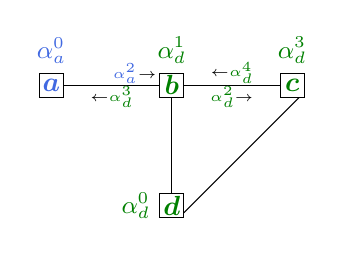
\begin{tikzpicture}[scale=0.87]

  \thickmuskip=0mu
  \medmuskip=0mu
  \thinmuskip=0mu
  
  \newcommand\X{50pt}
  \newcommand\Y{-50pt}

  \newcommand\ADD{\alpha}


  
  \draw (-\X + 5pt, 0) --
  node[above=-0.3em, right=-0.3em, above right, font=\tiny]{$\textcolor{\PA}{\ADD_a^2} \rightarrow$}
  node[below=-0.3em, font=\tiny]{$\leftarrow \textcolor{\PD}{\ADD_d^3}$}
  (0 - 5pt, 0); %% b - a 

  \draw (0 +5pt, 0) --
  node[above=-0.3em, font=\tiny]{$\leftarrow \textcolor{\PD}{\ADD_d^4}$}  
  node[below=-0.3em, font=\tiny]{$\textcolor{\PD}{\ADD_d^2} \rightarrow$}  
  (\X -5pt, 0); %% b - c

  \draw[opacity=0] (0, 0 - 5pt) --
  % node[opacity=1, above=-0.3em, font=\tiny, sloped]{$\ADD_{c}^{2} \rightarrow$}
  (0, \Y + 5pt); %% b - d
  \draw (0, \Y + 5pt) --
  % node[above=-0.3em, font=\tiny, sloped]{$\ADD_{c}^{2} \rightarrow$}
  (0, 0 - 5pt);  %% d - b
  
  \draw (\X + 3pt, 0 - 5pt) --
  % node[above=-0.3em, sloped, font=\tiny]{$\ADD_{c}^{2} \rightarrow$}
  (0 + 5pt, \Y - 3pt); %% c - d


  
  \draw[fill=white] (-\X, 0)
  node[color=\PA]{$\bm{a}$}
  +(-5pt, -5pt) rectangle +(5pt, 5pt);  
  \draw[fill=white] (0, 0)
  node[color=\PC]{$\bm{b}$}
  +(-5pt, -5pt) rectangle +(5pt, 5pt);
  \draw[fill=white] (\X, 0)
  node[color=\PC]{$\bm{c}$}
  +(-5pt, -5pt) rectangle +(5pt, 5pt);
  \draw[fill=white] (0, \Y)
  node[color=\PC]{$\bm{d}$}
  +(-5pt, -5pt) rectangle +(5pt, 5pt);

  \draw ( 0, 5pt) node[above, font=\small, color=\PD]{$\ADD_d^1$}; % b
  \draw ( \X, 5pt) node[above, font=\small, color=\PD]{$\ADD_d^3$}; % c
  \draw (-\X, 5pt) node[above, font=\small, color=\PA]{$\ADD_a^0$}; % a
  \draw (-5pt, \Y) node[left, font=\small, color=\PD]{$\ADD_d^0$}; % d
  
\end{tikzpicture}
}
    \hspace{5pt}
    \subfloat[Part D][\label{fig:addD}Processes $b$, $c$, and $d$ discard
      incoming messages. The system converged to optimal partitions.]{
      
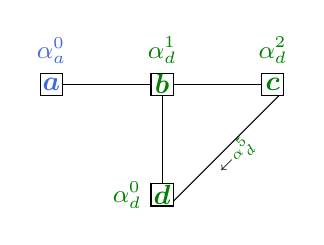
\begin{tikzpicture}[scale=0.8]

  \thickmuskip=0mu
  \medmuskip=0mu
  \thinmuskip=0mu
  
  \newcommand\X{50pt}
  \newcommand\Y{-50pt}

  \newcommand\ADD{\alpha}


  
  \draw (-\X + 5pt, 0) -- (0 - 5pt, 0); %% a - b

  \draw (0 +5pt, 0) --
  (\X -5pt, 0); %% b - c

  \draw (0, \Y + 5pt) --
  (0, 0 - 5pt);  %% d - b
  
  \draw (\X + 3pt, 0 - 5pt) --
  node[below=-0.3em, sloped, font=\tiny]{$\leftarrow \textcolor{\PD}{\ADD_{d}^{5}}$}
  (0 + 5pt, \Y - 3pt); %% c - d


  
  \draw[fill=white] (-\X, 0)
  node[color=\PA]{$\bm{a}$}
  +(-5pt, -5pt) rectangle +(5pt, 5pt);  
  \draw[fill=white] (0, 0)
  node[color=\PC]{$\bm{b}$}
  +(-5pt, -5pt) rectangle +(5pt, 5pt);
  \draw[fill=white] (\X, 0)
  node[color=\PC]{$\bm{c}$}
  +(-5pt, -5pt) rectangle +(5pt, 5pt);
  \draw[fill=white] (0, \Y)
  node[color=\PC]{$\bm{d}$}
  +(-5pt, -5pt) rectangle +(5pt, 5pt);
  
  \draw ( 0, 5pt) node[above, font=\small, color=\PD]{$\ADD_d^1$}; % b
  \draw ( \X, 5pt) node[above, font=\small, color=\PD]{$\ADD_d^2$}; % c
  \draw (-\X, 5pt) node[above, font=\small, color=\PA]{$\ADD_a^0$}; % a
  \draw (-5pt, \Y) node[left, font=\small, color=\PD]{$\ADD_d^0$}; % d

  
\end{tikzpicture}
}
    \caption{\label{fig:add}Simple accumulation in messages makes the
      system converge to consistent partitioning with scoped
      broadcast.}
  \end{center}
\end{figure*}

%%% Local Variables: 
%%% mode: latex
%%% TeX-master: "../paper"
%%% ispell-local-dictionary: "english"
%%% End: 

 

\begin{proof}
  When a \process $s_1$ becomes a source, it belongs to its own
  partition, for there exists no better partition than its own:
  $\forall p \in V: |\Pi_{s_1 s_1}| < |\Pi_{s_1 p}|$. It delivers,
  hence forwards such an $\alpha$ message to its neighbors. Since
  communication links are reliable, neighboring \processes eventually
  receive such a notification $\forall \langle s_1, q \rangle \in E,
  s_1 \in S \iff \eventually r_q(\alpha_{s_1}^{w_{s_1 q}})$. Most
  importantly, whatever the order of received messages, every \process
  $q'$ in this neighborhood -- such that there exists no better
  partition $s_2$ than the received one -- delivers and forwards it:
  $\forall s_2 \in S: |\Pi_{q' s_1}| < |\Pi_{q' s_2}| \implies
  \eventually d_{q'}(\alpha_{s_1}^{w_{s_1 q'}})$. By transitivity, the
  message originating from $s_1$ reaches all such \processes through
  their shortest paths: $\forall q'' \in V, s_1, s_2 \in S: |\Pi_{q''
    s_1}| < |\Pi_{q'' s_2}| \implies \eventually
  d_{q''}(\alpha_{s_1}^{|\Pi_{s_1 q''}|})$.  Since there exists only
  one best sum of weights per \process that can never be retracted,
  \processes eventually reach consistent partitioning.
  %% /!\ not equivalence for there exists other implementations.
  %% \item [$CP \implies BEF$:] By contradiction, if a \process $q \in
  %%   \Pi_{sp} = [s, \ldots, q, q', \ldots, p]$ with $s, q, p \in P_s$
  %%   does not forward its received $\alpha_s^{|\Pi_{sq}|}$, then
  %%   following \processes from $q'$ to $p$ may mistake another
  %%   partition for their  because it needs the weight $W_{pq}$.
  %% \end{asparadesc}
\end{proof}

\begin{algorithm}
  
\SetKwProg{Function}{func}{}{}

\small

\DontPrintSemicolon
\LinesNumbered

$O_p$ \tcp*[r]{set of neighbors and weights}
$d \leftarrow \infty$ \tcp*[r]{lowest distance to $q$}
$q$ \tcp*[r]{best partition}

\BlankLine

\Function{\textup{Add ( )}} {
  \textup{receiveAdd($p$, $0$)} \label{line:lowestbound}
}

\BlankLine

\Function{\textup{receiveAdd($q'$, $d'$)}} {
  \If { $d' < d$ } {
    $d \leftarrow d'$ \;
    $q \leftarrow q'$ \;

    \lForEach {$\langle n, w_n \rangle \in \mathcal{O}_p$} {
      \textup{send$_n$($q', d' + w_n$)} \label{line:accumulator}
    }
    
  }

}

  \caption{\label{algo:add}Adding a partition by \Process~$p$.}
\end{algorithm}

Algorithm~\ref{algo:add} shows the instructions that implement
consistent partitioning when
\begin{inparaenum}[(i)]
\item weights are scalar values,
\item \processes only add new partitions to the system,
\item and \processes never crash nor leave the system.
\end{inparaenum}
Figure~\ref{fig:add} illustrates its behavior on a system comprising 4
\processes $a$, $b$, $c$, and $d$. \Process~$a$ and \Process~$d$
become the sources of their partition. They \NAMEB a notification
\underline{a}dd message: $\alpha_a^0$ and $\alpha_d^0$. They
initialize their own state with the lowest possible bound $0$ (see
Line~\ref{line:lowestbound}), and send a message to each of their
neighbors by accumulating the corresponding edge weight (see
Line~\ref{line:accumulator}). In Figure~\ref{fig:addC}, \Process~$b$
receives $\alpha_{d}^{1}$. Since it improves its own partition
distance, it keeps it and forwards it to its neighbors. In
Figure~\ref{fig:addD}, \Process~$b$ discards $\alpha_{a}^{2}$, for it
does not improve its partition distance. \Processes $c$ and $d$ will
never acknowledge that Source~$a$ exists. Ultimately, \processes
discard last transiting messages. Despite the obvious lack of traffic
optimization, the system reaches consistent partitioning.

While only adding logical partitions to the distributed system is
straightforward, removing them introduces additional complexity caused
by concurrent operations.

\subsection{Dynamic consistent partitioning}
\label{subsec:dynamic}

%% At any time, a \process can become a source, hence adding a new
%% partition to the system. This partition eventually includes all
%% \processes that are closer from this new source than any other
%% else. \Processes naturally converge towards their respective best
%% partition by only piggybacking a monotonically increasing distance in
%% forwarded messages.

At any time, a source can revoke its self-appointed status of source
by executing a \texttt{Del} operation, hence deleting its partition
from the system. All \processes that belong to this partition must
eventually choose another partition to belong to. In
Figure~\ref{fig:del}, two partitions exist initially: $P_a$ and $P_d$
that respectively include $\{a\}$, and $\{b, c, d\}$. In
Figure~\ref{fig:delA}, \Process~$a$ deletes its partition. It notifies
all neighboring \processes~--~here only \Process~$b$~-- that may
belong to its partition using \NAMEB. Upon receipt, \Process~$b$
discards the \underline{d}elete notification $\delta_a$ since
$\delta_a$ does not target the former's partition $P_d$. \Process~$b$
sends its own best partition $\alpha_d^3$ that may be the best for
\Process~$a$. Eventually, every \process belongs to Partition
$P_d$. In this scenario, they reach consistent partitioning.

Delete operations add a new notion of order between events, and most
importantly between message deliveries. Delete operations implicitly
state that all preceding events become obsolete, and that all messages
originating from these preceding events convey stale control
information.

\begin{definition}[Happens-before $\rightarrow$~\cite{lamport1978time}]
  The transitive, irreflexive, and antisymmetric happens-before
  relationship defines a strict partial order between events. Two
  messages are concurrent if none happens before the other.
\end{definition}

\begin{definition}[\label{def:lwo}Message staleness]
  Only the latest message of a \process matters. A message $m$ conveys
  \underline{s}tale control information if the \process that broadcast
  $m$ later broadcast another message $m'$: $S(m) = \exists m': b_p(m)
  \rightarrow b_p(m')$.

  %% When a \process $p$ broadcasts two messages $b_p(m) \rightarrow
  %% b_p(m')$, no \process $q$ can deliver $m$ if it has delivered $m'$:
  %% $\nexists q \in V$ with $d_q(m') \rightarrow d_q(m)$, for $m$
  %% convey \emph{\underline{s}tale} control information: $S(m)$.
\end{definition}


\begin{figure}
  \begin{center}
    \subfloat[Part A][\label{fig:delA}Process~$a$ deletes its
      partition.  It notifies all processes that belong to its
      partition using \NAMEB.]{\input{input/figdelA.tex}}
    \hspace{5pt}
    %
    \subfloat[Part B][\label{fig:delB}$\delta$s stop as soon as they
      encounter another partition. Process~$b$ answers with its
      partition.]{
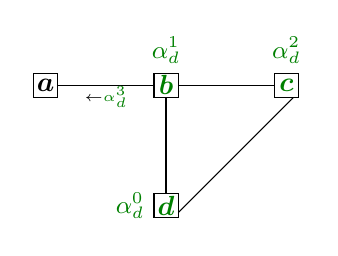
\begin{tikzpicture}[scale=0.87]

  \thickmuskip=0mu
  \medmuskip=0mu
  \thinmuskip=0mu
  
  \newcommand\X{50pt}
  \newcommand\Y{-50pt}

  \newcommand\ADD{\alpha}
  \newcommand\DEL{\delta}


  
  \draw (-\X + 5pt, 0) --
  node[below=-0.3em,font=\tiny]{$\leftarrow \textcolor{\PD}{\ADD_d^3}$}
  (0 - 5pt, 0); %% b - a 

  \draw (0 +5pt, 0) --
  (\X -5pt, 0); %% b - c

  \draw (0, 0 - 5pt) --
  (0, \Y - 5pt);  %% d - b
  
  \draw (\X + 3pt, 0 - 5pt) --
  (0 + 5pt, \Y - 3pt); %% c - d


  
  \draw[fill=white] (-\X, 0) node{$\bm{a}$} +(-5pt, -5pt) rectangle +(5pt, 5pt);  
  \draw[fill=white] (0, 0) node[color=\PD]{$\bm{b}$} +(-5pt, -5pt) rectangle +(5pt, 5pt);
  \draw[fill=white] (\X, 0) node[color=\PD]{$\bm{c}$} +(-5pt, -5pt) rectangle +(5pt, 5pt);
  \draw[fill=white] (0, \Y) node[color=\PD]{$\bm{d}$} +(-5pt, -5pt) rectangle +(5pt, 5pt);  

  \draw (0, 5pt) node[above, font=\small, color=\PD]{$\ADD_d^1$};
  \draw (\X, 5pt) node[above, font=\small, color=\PD]{$\ADD_d^2$};
  \draw (-5pt, \Y) node[left, font=\small, color=\PD]{$\ADD_d^0$};

  
\end{tikzpicture}
}
  \end{center}
  \caption{\label{fig:del}Efficient removal of a partition using
    \NAMEB. Process~$a$ eventually knows that it belong to Partition
    $P_d$.}
\end{figure}

%%% Local Variables: 
%%% mode: latex
%%% TeX-master: "../paper"
%%% ispell-local-dictionary: "english"
%%% End: 




\begin{figure*}
  \newcommand{\SCALE}{0.9}

  \newcommand{\SMSG}{\tiny}
  \newcommand{\OACK}{0.5}
  
  \thickmuskip=0mu
  \medmuskip=0mu
  \thinmuskip=0mu

  
  \newcommand\X{50pt}
  \newcommand\Y{-50pt}
 
  \newcommand{\LEFT}{\triangleleft}
  \newcommand{\RIGHT}{\triangleright}
  
  \begin{center}
    \subfloat[Part A][\label{fig:problemA}Both $a$ and $c$ become sources.
      $w_{ab} = 2$; $w_{bc} = 1$.]{\input{input/figsimplerproblemA.tex}}
    \hspace{0pt}
    \subfloat[Part B][\label{fig:problemB}Both $a$ and $c$ delete their partition 
     while $b$ delivers and forwards $\alpha_a$.]
             {\input{input/figsimplerproblemB.tex}}
    \hspace{0pt}
    \subfloat[Part C][\label{fig:problemC}$b$ blocks the only transiting
      $\delta_a$ while $b$ delivers and forwards $\alpha_c$.]
             {
\begin{tikzpicture}[scale=\SCALE]
  
  \draw (-\X + 5pt, 0) --
  node[above=-0.3em, font=\SMSG]{~ ~ ~ ~ ~ $\delta_{a} \RIGHT$} %% b - a
  node[above=-0.3em, font=\SMSG]{~ ~ ~ ~ ~ $\textcolor{\WRONG}{\text{\normalsize\xmark}} \hphantom{\RIGHT}$} %% b - a
  node[below=-0.3em, font=\SMSG]{$\LEFT \textcolor{\PC}{\alpha_c^3}$} %% b - a
  (0 - 5pt, 0);

  \draw [<->] (0 +5pt, 0) --
  node[opacity=\OACK, above=-0.3em, font=\SMSG]{$\alpha_c^2 \RIGHT$}
  node[below=-0.3em, font=\SMSG]{$\LEFT \delta_c \vphantom{\alpha^1}$~ ~ ~ ~ ~ ~}
  node[opacity=\OACK, below=-0.3em, font=\SMSG]{~ ~ ~ ~ ~ $\LEFT \alpha_a^4$}
  (\X -5pt, 0); %% b - c


  
  \draw[fill=white] (-\X, 0) node{$\bm{a}$} +(-5pt, -5pt) rectangle +(5pt, 5pt);  
  \draw[fill=white] (0, 0) node{\textcolor{\PC}{$\bm{b}$}} +(-5pt, -5pt) rectangle +(5pt, 5pt);
  \draw[fill=white] (\X, 0) node{\textcolor{\PA}{$\bm{c}$}} +(-5pt, -5pt) rectangle +(5pt, 5pt);
  
  \draw (-\X, 5pt) node[above, font=\scriptsize]{$\textcolor{\PA}{\alpha_a}\rightarrow \delta_a$};
  \draw (  0, 5pt) node[above, font=\scriptsize]{$\textcolor{\PA}{\alpha_a^2} \rightarrow \textcolor{\PC}{\alpha_c^1}$};
  \draw ( \X, 5pt) node[above, font=\scriptsize]{$\textcolor{\PC}{\alpha_c}\vphantom{\alpha_a^3} \rightarrow \delta_c \rightarrow \textcolor{\PA}{\alpha_a^3}$};


  %% \begin{scope}[shift={(0, -1*\Y)}]
  %%   \draw (-\X + 5pt, 0) --
  %%   node[below=-0.3em, font=\tiny]{$\LEFT \textcolor{\PC}{\alpha_c^3}$} %% b - a
  %%   (0 - 5pt, 0);
    
  %%   \draw (0 +5pt, 0) --
  %%   node[below=-0.3em, font=\tiny]{$\LEFT \delta_c \vphantom{\alpha^1}$}
  %%   (\X -5pt, 0); %% b - c
    
  %%   \draw[fill=white] (-\X, 0) node{\textcolor{\PA}{$\bm{a}$}} +(-5pt, -5pt) rectangle +(5pt, 5pt);  
  %%   \draw[fill=white] (0, 0) node{\textcolor{\PC}{$\bm{b}$}} +(-5pt, -5pt) rectangle +(5pt, 5pt);
  %%   \draw[fill=white] (\X, 0) node{\textcolor{\PA}{$\bm{c}$}} +(-5pt, -5pt) rectangle +(5pt, 5pt);
    
  %%   \draw (-\X, 5pt) node[above, font=\scriptsize]{$\textcolor{\PA}{\alpha_a^0}$};
  %%   \draw (  0, 5pt) node[above, font=\scriptsize]{$\textcolor{\PA}{\alpha_a^2} \rightarrow \textcolor{\PC}{\alpha_c^1}$};
  %%   \draw ( \X, 5pt) node[above, font=\scriptsize]{$\textcolor{\PC}{\alpha_c}\vphantom{\alpha_a^3} \rightarrow \delta_c \rightarrow \textcolor{\PA}{\alpha_a^3}$};
    
  %% \end{scope}

\end{tikzpicture}
}
    \hspace{0pt}
    \subfloat[Part D][\label{fig:problemD}$b$ delivers and forwards $\delta_c$. $c$
    stays in the deleted partition $P_a$.]
             {
\begin{tikzpicture}[scale=\SCALE]

  \thickmuskip=0mu
  \medmuskip=0mu
  \thinmuskip=0mu
  
  \newcommand\X{50pt}
  \newcommand\Y{-50pt}

  \newcommand\ADD{\alpha}
  \newcommand\DEL{\delta}


  
  \draw (-\X + 5pt, 0) --
  (0 - 5pt, 0);

  \draw [->] (0 +5pt, 0) --
  node[below=-0.3em, font=\tiny]{$\vphantom{\ADD^1_c }$}
  (\X -5pt, 0); %% b - c


  
  \draw[fill=white] (-\X, 0) node{$\bm{a}$} +(-5pt, -5pt) rectangle +(5pt, 5pt);  
  \draw[fill=white] (0, 0) node{$\bm{b}$} +(-5pt, -5pt) rectangle +(5pt, 5pt);
  \draw[color=\WRONG, fill=white] (\X, 0) node{\textcolor{\PA}{$\bm{c}$}} +(-5pt, -5pt) rectangle +(5pt, 5pt);
  
  \draw (-\X, 5pt) node[above, font=\scriptsize]{$\ldots \rightarrow \textcolor{\PC}{\ADD_c} \rightarrow \DEL_c$};
  \draw (  0, 5pt) node[above, font=\scriptsize]{$\ldots \rightarrow \DEL_c$};
  \draw ( \X, 5pt) node[above, font=\scriptsize]{$\ldots \rightarrow \textcolor{\PA}{\ADD_a^3}$};


  
  %% \begin{scope}[shift={(0, -1*\Y)}]

  %%   \draw (-\X + 5pt, 0) --
  %%   (0 - 5pt, 0);
    
  %%   \draw (0 +5pt, 0) --
  %%   node[below=-0.3em, font=\tiny]{$\vphantom{\ADD^1_c }$}
  %%   (\X -5pt, 0); %% b - c

    
  %%   \draw[fill=white] (-\X, 0) node{\textcolor{\PA}{$\bm{a}$}} +(-5pt, -5pt) rectangle +(5pt, 5pt);  
  %%   \draw[fill=white] (0, 0) node{\textcolor{\PA}{$\bm{b}$}} +(-5pt, -5pt) rectangle +(5pt, 5pt);
  %%   \draw[fill=white] (\X, 0) node{\textcolor{\PA}{$\bm{c}$}} +(-5pt, -5pt) rectangle +(5pt, 5pt);
    
  %%   \draw (-\X, 5pt) node[above, font=\scriptsize]{$\textcolor{\PA}{\ADD_a^0}$};
  %%   \draw (  0, 5pt) node[above, font=\scriptsize]{$\ldots \rightarrow \DEL_c \rightarrow \textcolor{\PA}{\ADD_a^2}$};
  %%   \draw ( \X, 5pt) node[above, font=\scriptsize]{$\ldots \rightarrow \textcolor{\PA}{\ADD_a^3}$};
  %% \end{scope}
  
\end{tikzpicture}
}
  \end{center}
  \caption{\label{fig:problem}Even in the simplest scenarios, naive
    propagation of $\alpha$ and $\delta$ messages may be insufficient
    to guarantee consistent partitioning. In the bottom scenario, if
    $c$ had children, they would stay in the wrong partition
    too.
    %
    % Despite both scenarios look the same from $c$'s perspective, $c$
    % must acknowledge $P_a$'s \emph{possible} deletion and propagate
    % it.
  }
\end{figure*}



Unfortunately, stale control information as stated in
Definition~\ref{def:lwo} may impair the propagation of both
\begin{inparaenum}[(i)]
\item notifications about actual sources, and
\item notifications about deleted partitions.
\end{inparaenum}
\TODO{Rework here.}
Figure~\ref{fig:problem} highlights such consistency issues with
dynamic partitions, even in contexts where \processes have FIFO links,
\ie where \processes receive the messages in the order of their
sending ($s_{pq}(m) \rightarrow s_{pq}(m') \implies r_q(m) \rightarrow
r_q(m')$). Both $a$ and $d$ add then delete their partition
concurrently. \Process~$c$ receives, delivers, and forwards
$\alpha_d^3$ followed by $\delta_d$. In the meantime, $b$ receives,
delivers, and forwards $\alpha_a^2$. In Figure~\ref{fig:problemC},
both $c$ and $d$ deliver the message about Partition $P_a$, for they
did not have any known partition at receipt time. On the contrary, $b$
delivers $\alpha_d^1$, for it improves its distance to a known
source. \Process~$b$ then blocks $a$'s removal notification
$\delta_a$. It never reaches $c$ nor $d$. Also, $c$ does not deliver
$\alpha_d$ and $\delta_d$ since it already delivered it. The system
converges to an inconsistent state where some \processes assume they
belong to a partition while it does not exist anymore. The system
needs to purge stale $\alpha$ messages that stop $\delta$ messages
from reaching nodes.

\begin{definition}[\label{def:purge}Message purge]
  A system purges a message $P(m)$ when every \node $q$ that delivered
  $m$ eventually delivers another message $m'$ never followed by the
  delivery of the former message $m$: $d_q(m) \implies \eventually
  (d_q(m) \rightarrow d_q(m'))$.
\end{definition}


\begin{theorem}[\label{theo:dcp}EFB$^+$: EFB $\wedge$ (Purge $\rightarrow$ EFB) $\implies$
    \underline{D}ynamic \underline{c}onsistent
    \underline{p}artitioning (DCP)]
%
  When a \process can \texttt{Add} and \texttt{Del}ete its partition,
  to ensure consistent partitioning, eventual forwarding of best
  (Theorem~\ref{theo:efb}) additionally requires
\begin{inparaenum}[(i)]
\item eventual purging of stale messages ($S(m) \implies P(m)$), then
\item the eventual forwarding of best (Definition~\ref{theo:efb}).
\end{inparaenum}
\end{theorem}

\begin{proof}
  %% To reach consistent partitioning, the last message delivered by
  %% every process is not stale and comes from its respective best
  %% source: $d(m)$
  Assuming EFB as default propagation behavior where \processes
  deliver and forward the best sum of weights they received. We must
  prove that despite stale messages, the last delivery of every
  \process is the message that followed the shortest path to its
  closest source.
  \begin{asparadesc}
  \item [EFB without Purge:] From Figure~\ref{fig:problemD}, a
    \process may receive messages in such an order ($d_b(\alpha_d^1)
    \rightarrow r_b(\delta_a) \rightarrow d_b(\delta_d)$) that it does
    not forward messages required by other \processes
    ($\delta_a$). The last delivery of some nodes ($c$ and $d$) is
    wrong ($\alpha_a^3$ instead of $\delta_a$).
    % \Processes never
    % reach consistent partitioning.
    %
    %% Figure~\ref{fig:proofA} depicts the generic case where a \process
    %% $b$ precludes itself and subsequent \processes such as $c$ of
    %% delivering the message from their respective best source
    %% $a$. \Process $b$ received and delivered a message from a
    %% partition that has since then been deleted but with a better sum
    %% of weights than newly received ones ($\alpha_d^y <
    %% \alpha_a^{x'}$). It forever discards such a message
    %% $\alpha_a^{x'}$.
  \item [Purge not followed by EFB:]
    %% also transiting messages
    Assuming that every \process removes control information as soon
    as it becomes stale ($S(\alpha_a) \implies d_b(\alpha_a^x)
    \rightarrow d_b(\delta_a)$) and cannot deliver stale messages
    anymore ($S(\alpha_a^x) \implies d_c(m) \rightarrow \ldots
    \rightarrow d_c(m' \not\in \alpha_a)$), staleness does not impair
    up-to-date messages propagation. However, even in such settings,
    depending on receipt order ($d_b(\alpha_a^{x}) \rightarrow
    r_b(\alpha_c^{y : y > x}) \rightarrow d_b(\delta_b)$), a \process
    may never receive again, hence deliver and forward a message that
    was received and discarded before ($\alpha_c^{y}$). When such a
    message contains its best up-to-date partition, a \process may
    never end up in its best partition.
    %    Therefore, \processes do not reach
    % consistent partitioning.
  \item [Purge then EFB:] Assuming the eventual and definitive removal
    of stale messages at each \process ($S(\alpha_a) \implies
    (d_b(\alpha_a) \implies \eventually d_b(\alpha_a) \rightarrow
    d_b(m') \not\rightarrow d_b(\alpha_a))$); and assuming that every
    removal eventually triggers the forwarding of best delivered
    messages ($d_c(\delta_x) \implies \eventually f_d(\alpha_y)$),
    \processes may deliver other stale messages that will be 
    eventually removed to never be delivered again. In the worst case,
    all \processes deliver and remove all stale messages to ultimately
    deliver and forward only up-to-date messages ($\eventually d_c(m')
    \implies \neg S(m')$). As in Theorem~\ref{theo:efb}, they
    eventually deliver and forward their best up-to-date message.
    
    %% upon receipt of such $\alpha_y$, either the \process already
    %% delivered its removal and it does 
    

    %% ($d_c(\delta_x) \implies \eventually f_d(\alpha_y) \wedge \neg
    %% S(\alpha_y)$)


    %% eventually every \process only delivers and forwards up-to-date
    %% messages, or no message at all 




    %% , every \process eventually delivers and forwards the best
    %% up-to-date delivered messages as in Theorem~\ref{theo:bef}.
    
    %% Removing \emph{forever} all such stale messages about
    %% deleted partitions would allow \processes to propagate their best
    %% up-to-date partition again, eventually reaching consistent
    %% partitioning together, as stated by Theorem~\ref{theo:bef}.
  \end{asparadesc}
  Using EFB$^+$, \processes reach consistent partitioning together
  even under dynamic partitioning settings where \nodes can
  \texttt{Add} and \texttt{Del}ete their partition.
\end{proof}

%% Figure removed as it's kind of redundant with preceding figure that
%% depicts the issue
%% \begin{figure} 
%%   \centering
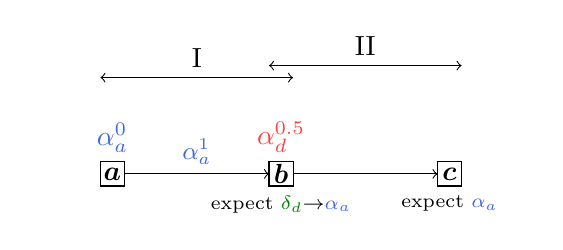
\begin{tikzpicture}[scale=0.87]

  \thickmuskip=0mu
  \medmuskip=0mu
  \thinmuskip=0mu
  
  \newcommand\X{70pt}
  \newcommand\Y{-40pt}

  \newcommand\ADD{\alpha}
  \newcommand\DEL{\delta}

  \draw[opacity=0] (-1.5*\X, 0) -- (1.5*\X, 0);
  


  \draw[<->] (-5pt - \X, -\Y) -- node[above]{I} (5pt, -\Y); %% I
  
  \draw[->] (-\X + 5pt, 0) --
  node[above, color=\PA, font=\small]{$\ADD_a^1$}
  (0 - 5pt, 0); %% a - b

  \draw[<->] (-5pt, 5pt -\Y) -- node[above]{II} (5pt + \X, 5pt -\Y); %% II
  \draw[->] (0 + 5pt, 0) -- (-5pt +  \X, 0); %% b - c


  
  \draw[fill=white] (-\X, 0) node{$\bm{a}$} +(-5pt, -5pt) rectangle +(5pt, 5pt);  
  \draw[fill=white] (0, 0) node{$\bm{b}$} +(-5pt, -5pt) rectangle +(5pt, 5pt);
  \draw[fill=white] (\X, 0) node{$\bm{c}$} +(-5pt, -5pt) rectangle +(5pt, 5pt);


  
  \draw (-\X, 5pt) node[above, color=\PA]{$\ADD_a^0$};
  \draw ( 0, 5pt) node[above, color=\WRONG]{$\ADD_d^{0.5}$};
  \draw (\X,-5pt) node[below, font=\scriptsize]{expect \textcolor{\PA}{$\alpha_a$}};
  \draw (0, -5pt) node[below, font=\scriptsize]{expect $\textcolor{\PC}{\DEL_d} \rightarrow \textcolor{\PA}{\alpha_a}$};

\end{tikzpicture}

%%   \caption{\label{fig:proofA}Stale $\alpha$ messages may
%%       stop other $\alpha$ messages from reaching all \processes ($b$
%%       and $c$) that require it along the shortest path. Consistent
%%       partitioning requires eventual purging of stale messages (see
%%       Figure~\ref{fig:proofB}).}
%% \end{figure}

The main challenge consists in implementing a purging mechanism that
ensures the \emph{eventual and definitive} removal of stale control
information. One could guarantee consistent partitioning by always
propagating the $\delta$ messages corresponding to the $\alpha$
messages it propagated before. In Figure~\ref{fig:problem}, it means
that as soon as \Process~$b$ forwards $\alpha_a^2$, it assumes that
its neighbors \Process~$c$ and \Process~$d$ may need the notification
of removal $\delta_a$ if it exists. However, such a solution also
implies that \processes generate traffic not only related to their
current partition, but also related to partitions they belonged to in
the past. This would prove overly expensive in dynamic systems where
\processes join and leave the system, create and delete partitions, at
any time.  Instead, we propose to use the delivery order at each
\process to detect possible inconsistencies and solve them.
%% Together, \processes eventually remove all stale control information
%% (transiting messages and local states) of the system leaving room for
%% propagation of messages about up-to-date partitions.

%% 
\begin{figure*}
  \begin{center}
    \subfloat[Part A][\label{fig:proofA}Stale $\alpha$ messages may
      stop other $\alpha$ messages from reaching all \processes ($b$
      and $c$) that require it along the shortest path. Consistent
      partitioning requires eventual purging of stale messages (see
      Figure~\ref{fig:proofB}).]  {
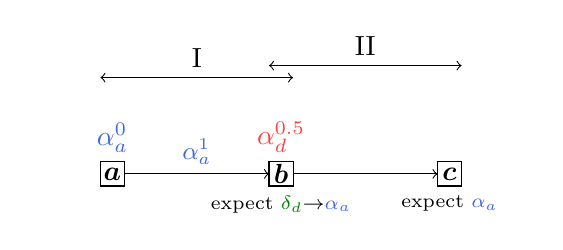
\begin{tikzpicture}[scale=0.87]

  \thickmuskip=0mu
  \medmuskip=0mu
  \thinmuskip=0mu
  
  \newcommand\X{70pt}
  \newcommand\Y{-40pt}

  \newcommand\ADD{\alpha}
  \newcommand\DEL{\delta}

  \draw[opacity=0] (-1.5*\X, 0) -- (1.5*\X, 0);
  


  \draw[<->] (-5pt - \X, -\Y) -- node[above]{I} (5pt, -\Y); %% I
  
  \draw[->] (-\X + 5pt, 0) --
  node[above, color=\PA, font=\small]{$\ADD_a^1$}
  (0 - 5pt, 0); %% a - b

  \draw[<->] (-5pt, 5pt -\Y) -- node[above]{II} (5pt + \X, 5pt -\Y); %% II
  \draw[->] (0 + 5pt, 0) -- (-5pt +  \X, 0); %% b - c


  
  \draw[fill=white] (-\X, 0) node{$\bm{a}$} +(-5pt, -5pt) rectangle +(5pt, 5pt);  
  \draw[fill=white] (0, 0) node{$\bm{b}$} +(-5pt, -5pt) rectangle +(5pt, 5pt);
  \draw[fill=white] (\X, 0) node{$\bm{c}$} +(-5pt, -5pt) rectangle +(5pt, 5pt);


  
  \draw (-\X, 5pt) node[above, color=\PA]{$\ADD_a^0$};
  \draw ( 0, 5pt) node[above, color=\WRONG]{$\ADD_d^{0.5}$};
  \draw (\X,-5pt) node[below, font=\scriptsize]{expect \textcolor{\PA}{$\alpha_a$}};
  \draw (0, -5pt) node[below, font=\scriptsize]{expect $\textcolor{\PC}{\DEL_d} \rightarrow \textcolor{\PA}{\alpha_a}$};

\end{tikzpicture}
}
    \hspace{10pt}
    \subfloat[Part B][\label{fig:proofB}Stale $\alpha$ messages may
      stop $\delta$ messages from reaching processes with the corresponding
      partition. Consistent partitioning requires that all \processes propagate
      $\delta$ messages as often as possible (I'); detect possible inconsistencies
      when parents' $\alpha$ messages contradict delivery history or state (III); notify
      processes of possible inconsistencies (IV).]
    {
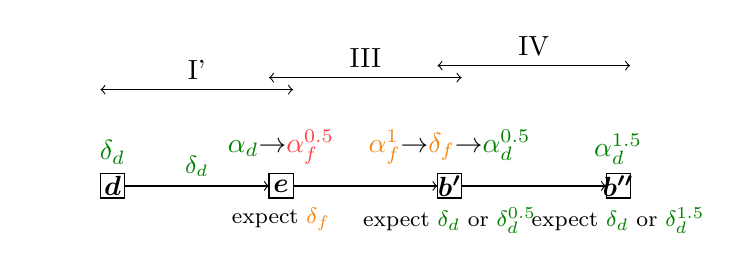
\begin{tikzpicture}[scale=0.87]

  \thickmuskip=0mu
  \medmuskip=0mu
  \thinmuskip=0mu
  
  \newcommand\X{70pt}
  \newcommand\Y{-40pt}

  \newcommand\ADD{\alpha}
  \newcommand\DEL{\delta}

  \draw[opacity=0] (-1.5*\X, 0) -- (2.5*\X, 0);
  


  \draw[<->] (-5pt - \X, -\Y) -- node[above]{I'} (5pt, -\Y); %% I as well
  \draw[->] (-\X + 5pt, 0) -- node[above, font=\small, color=\PC]{$\DEL_d$} (0 - 5pt, 0); %% d - e

  \draw[<->] (-5pt , 5pt -\Y) -- node[above]{III} (5pt + \X, 5pt -\Y); %% IV
  \draw[->] (0 +5pt, 0) -- (\X -5pt, 0); %% e - b'
  
  \draw[<->] (-5pt + \X , 10pt -\Y) -- node[above]{IV} (5pt + 2*\X, 10pt -\Y); %% V
  \draw[->] ( \X +5pt, 0) -- (2*\X -5pt, 0); %% b - b''


  
  \draw[fill=white] (-\X, 0) node{$\bm{d}$} +(-5pt, -5pt) rectangle +(5pt, 5pt);  
  \draw[fill=white] (0, 0) node{$\bm{e}$} +(-5pt, -5pt) rectangle +(5pt, 5pt);
  \draw[fill=white] (\X, 0) node{$\bm{b'}$} +(-5pt, -5pt) rectangle +(5pt, 5pt);
  \draw[fill=white] (2*\X, 0) node{$\bm{b''}$} +(-5pt, -5pt) rectangle +(5pt, 5pt);


  
  \draw (-\X, 5pt) node[above, color=\PC]{$\DEL_d$};
  
  \draw ( 0, 5pt) node[above]{$\textcolor{\PC}{\ADD_d} \rightarrow \textcolor{\WRONG}{\ADD_f^{0.5}}$};
  \draw ( 0, -5pt) node[below, font=\footnotesize]{expect $\textcolor{\PB}{\DEL_f}$};
  
  \draw ( \X, 5pt) node[above]{$\textcolor{\PB}{\ADD_f^1} \rightarrow \textcolor{\PB}{\DEL_f} \rightarrow \textcolor{\PC}{\ADD_d^{0.5}}$};
  \draw ( \X, -5pt) node[below, font=\footnotesize]{expect $\textcolor{\PC}{\DEL_d}$ or $\textcolor{\PC}{\DEL_d^{0.5}}$};

  \draw (2*\X, 5pt) node[above]{$\textcolor{\PC}{\ADD_d^{1.5}}$};
  \draw (2*\X, -5pt) node[below, font=\footnotesize]{expect $\textcolor{\PC}{\DEL_d}$ or $\textcolor{\PC}{\DEL_d^{1.5}}$};
  
\end{tikzpicture}
}
    \caption{\label{fig:proof}Concurrent operations,
      delivery orders, and stale control information may impair
      consistent partitioning. Dynamic consistent partitioning
      requires eventual purging of stale messages, and best eventual
      forwarding.}
  \end{center}
\end{figure*}

%%% Local Variables: 
%%% mode: latex
%%% TeX-master: "../paper"
%%% ispell-local-dictionary: "english"
%%% End: 



%% Figure~\ref{fig:proof} depicts the issues with staleness and message
%% orderings. In Figure~\ref{fig:proofA}, the shortest path from any
%% source to \Process $c$ is $[a, b, c]$. However, \Process $b$ still holds
%% a stale $\alpha_d^{0.5}$ without knowing. When it receives
%% $\alpha_a^1$, it discards it, for it assumes that downstream \processes
%% are more interested in $\alpha_d^{0.5}$. To reach consistent
%% partitioning, \Process $b$ first needs to purge its current partition
%% to later accept that of its current actual shortest path:
%% $\alpha_a^1$.

%% \noindent Figure~\ref{fig:proofB} shows that removing stale control
%% information is even more complex. The removal must reach all \processes
%% of the previous shortest path going from $d$ to $b''$. Label I' shows
%% the most obvious issue where \Process $e$ changed partition for a
%% better but stale $\alpha_f$. Since it can remember its previous
%% deliveries, it could still forward $\delta_d$ for the sake of
%% consistency. However, this would lead to every \process forwarding
%% every $\delta$ they ever delivered. Such protocol's overhead would
%% depend on past partitioning instead of current one. Label III shows
%% the issue when the blocking partition is already known to be stale at
%% \Process $b'$. \Process $b''$ eventually receives $\alpha_f$ from
%% $e$. However, it cannot deliver it, for it would break last win order.
%% \Process $b'$ may be in an inconsistent state. Label IV shows the
%% corollary issue: \Process $b''$ delivered a message from a \process that
%% may be inconsistent without knowing it.

\begin{theorem}[\label{theo:threephase}Three-phase purge]
  Three phases are sufficient to eventually purge the system from
  stale control information:
  \begin{inparaenum}[(i)]
  \item propagation of delete notifications,
  \item detection of possibly blocking conditions, and
  \item propagation of delete notifications that were possibly blocked.
  \end{inparaenum}
\end{theorem}

%% \begin{figure}
%%   \centering
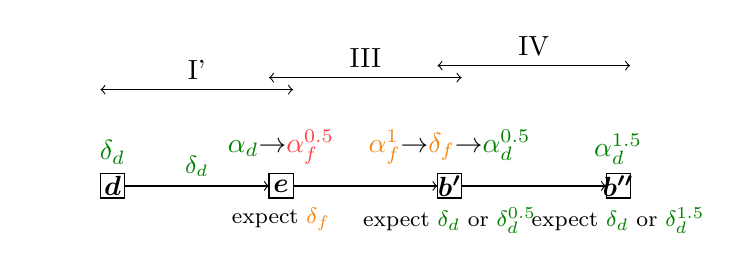
\begin{tikzpicture}[scale=0.87]

  \thickmuskip=0mu
  \medmuskip=0mu
  \thinmuskip=0mu
  
  \newcommand\X{70pt}
  \newcommand\Y{-40pt}

  \newcommand\ADD{\alpha}
  \newcommand\DEL{\delta}

  \draw[opacity=0] (-1.5*\X, 0) -- (2.5*\X, 0);
  


  \draw[<->] (-5pt - \X, -\Y) -- node[above]{I'} (5pt, -\Y); %% I as well
  \draw[->] (-\X + 5pt, 0) -- node[above, font=\small, color=\PC]{$\DEL_d$} (0 - 5pt, 0); %% d - e

  \draw[<->] (-5pt , 5pt -\Y) -- node[above]{III} (5pt + \X, 5pt -\Y); %% IV
  \draw[->] (0 +5pt, 0) -- (\X -5pt, 0); %% e - b'
  
  \draw[<->] (-5pt + \X , 10pt -\Y) -- node[above]{IV} (5pt + 2*\X, 10pt -\Y); %% V
  \draw[->] ( \X +5pt, 0) -- (2*\X -5pt, 0); %% b - b''


  
  \draw[fill=white] (-\X, 0) node{$\bm{d}$} +(-5pt, -5pt) rectangle +(5pt, 5pt);  
  \draw[fill=white] (0, 0) node{$\bm{e}$} +(-5pt, -5pt) rectangle +(5pt, 5pt);
  \draw[fill=white] (\X, 0) node{$\bm{b'}$} +(-5pt, -5pt) rectangle +(5pt, 5pt);
  \draw[fill=white] (2*\X, 0) node{$\bm{b''}$} +(-5pt, -5pt) rectangle +(5pt, 5pt);


  
  \draw (-\X, 5pt) node[above, color=\PC]{$\DEL_d$};
  
  \draw ( 0, 5pt) node[above]{$\textcolor{\PC}{\ADD_d} \rightarrow \textcolor{\WRONG}{\ADD_f^{0.5}}$};
  \draw ( 0, -5pt) node[below, font=\footnotesize]{expect $\textcolor{\PB}{\DEL_f}$};
  
  \draw ( \X, 5pt) node[above]{$\textcolor{\PB}{\ADD_f^1} \rightarrow \textcolor{\PB}{\DEL_f} \rightarrow \textcolor{\PC}{\ADD_d^{0.5}}$};
  \draw ( \X, -5pt) node[below, font=\footnotesize]{expect $\textcolor{\PC}{\DEL_d}$ or $\textcolor{\PC}{\DEL_d^{0.5}}$};

  \draw (2*\X, 5pt) node[above]{$\textcolor{\PC}{\ADD_d^{1.5}}$};
  \draw (2*\X, -5pt) node[below, font=\footnotesize]{expect $\textcolor{\PC}{\DEL_d}$ or $\textcolor{\PC}{\DEL_d^{1.5}}$};
  
\end{tikzpicture}

%%   \caption{\label{fig:proofB}Stale $\alpha$ messages may stop $\delta$
%%     messages from reaching \processes with the corresponding
%%     partition. Consistent partitioning requires that all \processes
%%     propagate $\delta$ messages as often as possible (I); detect
%%     possible inconsistencies when parents' $\alpha$ messages
%%     contradict history or state (II); notify \processes of possible
%%     inconsistencies (III).}
%% \end{figure}

\begin{proof}
  We must prove that every \process that delivered a stale $\alpha_X$
  eventually delivers a better $\alpha_Y$, or delivers a removal
  notification of $\alpha_X$.  Figure~\ref{fig:proofB} summarizes the
  issue of purging in scenarios involving concurrent operations.

  
  (i) If every \process (such as $a$) starting from the source
  delivers and forwards a removal notification $\delta_X$ when their
  last delivery is $\alpha_X$, then every such \process eventually
  delivers the removal notification $\delta_X$ except \processes (such
  as $b$) that delivered $\alpha_X$ from a \process that delivered a
  message from another partition $\alpha_Y$ since then.
  
  These exceptions eventually receive and deliver $\alpha_Y$ since
  $\alpha_Y$ is better than $\alpha_X$ through this path, except if
  they already received and delivered the removal notification of
  $P_Y$ (such as $c$). These \processes may never receive hence
  deliver $\delta_X$, and may never receive hence deliver a better
  message than $\alpha_X$. They need an additional mechanism to
  eventually purge $\alpha_X$ that cannot rely on the eventual purging
  of $P_Y$ at \processes like $b$, to avoid deadlocks.
  
  (ii) Assuming that every \process keeps an history of its past
  deliveries, \processes (such as $c$) can detect the inconsistency,
  since they receive from their parent an already deleted partition
  $P_Y$. This notification means that the parent discards any
  $\delta_Z$ with $\alpha_Z^z < \alpha_Y^y$, and most importantly, if
  $\delta_X$ exists, it discards it. To ensure the purge of stale
  messages, a detecting \process must assume the worst case that such
  $\delta_X$ exists, and send another kind of message, noted $\Delta$,
  that notify the possible removal of $P_X$.
  
  (iii) A \process (such as $d$) whose last delivery is $\alpha_X$,
  but whose parent is neither inconsistent (like $b$) nor receiving
  $\delta_X$ (like $a$), eventually receives $\Delta$ from a detecting
  \process, either directly or transitively, for such a child \process
  ($d$) trusts the possible removal of $P_X$ by delivering and
  forwarding such $\Delta$. $\Delta$ suffers from identical blocking
  conditions (between $b$ and $c$) than $\delta$, leading to the same
  solutions of detection and propagation of $\Delta$. Eventually,
  every \process whose last delivery is $\alpha_X$ receives and
  delivers either a better $\alpha_Z$, or $\delta_X$, or $\Delta_X$.
  %
  %% Some \processes may have delivered messages about other partitions
  %% before or after $\alpha_X$. \Processes such as $b$ and $c$ delivered
  %% messages about $P_Y$.  For \processes such as $b$, the last delivery
  %% is $\alpha_Y$: $d_b(\_) \rightarrow \ldots \rightarrow d_b(\alpha_X)
  %% \rightarrow \ldots \rightarrow d_b(\alpha_Y)$; For \processes such
  %% as $c$, the last delivery is $\alpha_X$, and they delivered the
  %% addition and removal of $P_Y$: $d_c(\_) \rightarrow \ldots
  %% \rightarrow d_c(\alpha_Y) \rightarrow \ldots \rightarrow
  %% d_c(\delta_Y) \rightarrow \ldots \rightarrow d_c(\alpha_X)$. Both
  %% $a$ and $d$ delivered $\alpha_X$ last: $d_a(\_) \rightarrow \ldots
  %% \rightarrow d_a(\alpha_X)$. Their difference being their position in
  %% the chain: $d$ is a child of \processes that delivered messages
  %% about $P_Y$.
  %
  %% \begin{asparadesc}
  %% \item [($a$ or $c$ or $d$) to ($a$ or $c$ or $d$):] The source is
  %%   like $a$.  By propagating from \process to \process the
  %%   corresponding $\delta_X$ message, these \processes purge
  %%   $\alpha_X$.
  %% \item [$a$ to $b$:] $b$ stops the propagation of $\delta_X$, for the
  %%   latter does not target its current partition.
  %% \item [$b$:] They need to purge their own $P_Y$, we must \TODO{prove
  %%   that $[a, b, c, d]$ is solved and that it does not require to
  %%   purge $P_Y$.}
  %% \item [$b$ to $d$:] would deliver $d_(\alpha_y)$ hence becoming $b$.
  %% \item [$b$ to $c$:] block $d_c(\alpha_y)$, so $c$ stays in $c$. But
  %%   it detects $b$ is its parent, and possibly blocked any delta with
  %%   its value $r_b(\delta_z) \rightarrow d_b(\delta_z)$. Since not
  %%   sure, $\Delta$
  %
  %% \item [\processes with $\alpha_X^x \rightarrow \alpha_Y^y$ with last
  %%   $\alpha_Y^y$, for $\alpha_Y^y< \alpha_X^x$:] \Processes such as
  %%   \Process~$b$ that do not directly suffer from the non-delivery of
  %%   $\delta_X$. They need to purge their own $P_Y$ if need
  %%   be. Nonetheless, they deliver and forward $\alpha_Y$ that at least
  %%   one following \process will receive.
  %% \item [\processes with $\delta_Y \rightarrow \alpha_X$:] \Processes
  %%   such as \Process~$c$ that do not belong to the preceding category,
  %%   for they already delivered $\delta_Y$. Nevertheless, best eventual
  %%   forwarding guarantees that they receive $\alpha_Y$, which
  %%   contradicts their history or state. In such a case, the detecting
  %%   \processes purge their own $\alpha_X$. The detecting \processes
  %%   must also notify subsequent \processes that their current
  %%   partition \emph{may be} deleted. Indeed their parent may have
  %%   blocked the corresponding $\delta$ messages and subsequent
  %%   \processes must purge their possibly stale state, for the sake of
  %%   consistency.  We note such a notification $\Delta_X$ to emphasize
  %%   their proximity to $\delta_X$ messages.
  %%   % the uncertainty of a $\delta$ message.
  %% \item [\processes with last $\alpha_X$ receiving $\Delta_X$ from
  %%   their parent:] \Processes such as \Process~$d$ that have
  %%   $\alpha_X$ but preceding delivered messages are not
  %%   important. Such \processes must trust detecting \processes by
  %%   delivering and forwarding $\Delta_X$. It is worth noting that
  %%   these messages are subject to all aforementioned blocking
  %%   conditions, but are also solved by aforementioned mechanisms.
  %% \end{asparadesc}
  %% Propagation~I terminates: a \process does not deliver a $\delta$
  %% message if it has already delivered it. Propagation~III terminates: a
  %% \process does not deliver a looping message.  
  % ; and since \processes forward the messages they deliver, upstream
  % \processes eventually receive and may deliver messages detected as
  % issue. In Figure~\ref{fig:proofB}, \Process~$e$ eventually
  % receives $\delta_f$ from \Process~$b'$.
  %% Three-phase purge ensures that all \processes of the system
  %% eventually removes stale messages, leaving room for best eventual
  %% forwarding of up-to-date messages.
  %
  %  \TODO{cannot loop add from $e$ , undo from $b'$ because $b'$ sent
  % delete to $e$, it will solve the inconsistency.}
  %
  %% In the meantime, \processes that still belong to a partition can
  %% propagate their respective last $\alpha$ message, and reach
    %% consistent partitioning.
\end{proof}



\subsection{Implementation and complexity}

Algorithm~\ref{algo:ascast} provides the few instructions of \NAME
that implement three-phase purge and eventual forwarding of best to
enable dynamic consistent partitioning. For the sake of simplicity, it
does not handle multiple sessions and associated optimisation such as
data structure sharing and message packing.

\begin{algorithm}
  
\SetKwProg{Function}{func}{}{}

\small

\DontPrintSemicolon
\LinesNumbered

$O_p$, $W_p$ \tcp*[r]{set of neighbors and weights}
$A_{s, c}^{d, \pi} \leftarrow \alpha_{\infty, 0}^{\infty, \varnothing} $ \tcp*[r]{best $\alpha$ so far}
$V \leftarrow \varnothing$;~ $V[p] \leftarrow 0$ \tcp*[r]{vector of versions}

\BlankLine
\BlankLine

\Function{\textup{Add ( )}} { % \hfill [if $V[p]\equiv 0 \mod 2 $]} } {
  \textup{\smash{receiveAdd($p$, $\alpha_{p, V[p] + 1}^{0, \varnothing}$)}}\label{line:ascast_add}
}

\BlankLine

\Function{\textup{Del ( )}} { % \hfill [if $V[p]\equiv 1 \mod 2 $]} } {
  \textup{\smash{receiveDel($p$, $\delta_{p, V[p] + 1}$)}}\label{line:ascast_del}
}

\BlankLine
\BlankLine

\Function{\textup{receiveAdd($q$, $\alpha_{s', c'}^{d', \pi'}$)}
\tcp*[f]{\footnotesize{receive $\alpha$ from $q$}}} {
    \uIf(\tcp*[f]{\footnotesize{or state}}) {\hphantom{$($}$q = \pi[|\pi| - 1] \, \wedge$\tcp*[f]{{\footnotesize{from parent: III detect}}}\\
    \hphantom{\textbf{if}} $(c' < V[s'] \,  \vee$\tcp*[f]{\footnotesize{inconsistent version}\label{line:ascast_version}}\\
    \hphantom{\textbf{if}} \smash{$(\alpha_{s', c'}^{d', \pi'} < A_{s, c}^{d, \pi} \wedge p\not\in \pi'))$}\label{line:detectA}} {
        \textup{receiveDel($q$, $\delta_{s, c}^{\pi}$)} \tcp*[r]{\footnotesize{IV propagate}}
    }
    \uElseIf (\tcp*[f]{\footnotesize{I propagate}\label{line:ascast_better}}) {$A_{s, c}^{d, \pi} < \alpha_{s', c'}^{d', \pi} \wedge p \not\in \pi'$  } {
          $V[s'] \leftarrow c'$ \;
          $A_{s, c}^{d, \pi} \leftarrow \alpha_{s', c'}^{d', \pi'}$ \;
              \lForEach{$n \in O_p$}
                  {\smash{send$_n$($\alpha_{s', c'}^{d' + W_{pq}, \pi' \cup p}$)}}

     }
}



\BlankLine

\Function{\textup{receiveDel($q$, $\delta_{s', c'}^{\pi'}$)}
\tcp*[f]{\footnotesize \smash{$r_p (\delta_{s', c'})$ \textup{\texttt{or}} $r_p (\delta_{s', c'}^{\pi'})$}}} {
  \uIf {$((\delta_{s', c'} \wedge \alpha_{s', c'-1} = A_{s, c}) \, \vee$\tcp*[f]{\footnotesize{I' propagate}}\\
    \hphantom{\textbf{if} } $(\delta_{s',c'}^{\pi'} \wedge \alpha_{s', c'}^{\_, \pi'} = A_{s, c}^{\_, \pi})) \, \wedge$\tcp*[f]{\footnotesize{IV propagate}}\\
    \hphantom{\textbf{if} $($} $p \not\in \pi'$ \label{line:notloopingB}} {
     $V[s'] \leftarrow \max(V[s'], c')$ \;
     $A_{s, c}^{d, \pi} \leftarrow \alpha_{\infty, 0}^{\infty, \varnothing}$ \;


     \ForEach{$n \in O_p$}{
       \lIf {\smash{$\delta_{s', c'}^{\pi'}$}} {send$_n$(\smash{$\delta_{s', c'}^{\pi' \cup p}$)}
       \textbf{else} send$_n$(\smash{$\delta_{s', c'}$)} }
     }

  }\uElseIf{$A_{s, c}^{d, \pi} \neq \alpha_{\infty, 0}^{\infty, \varnothing}$} {
     \textup{send$_q$($\alpha_{s, c}^{d + W_{pq}, \pi \cup p}$)}
     \tcp*[r]{\label{line:ascast_compete}\footnotesize{compete}}
  }
}

%%% Local Variables: 
%%% mode: latex
%%% TeX-master: "../paper"
%%% ispell-local-dictionary: "english"
%%% End: 

  \caption{\label{algo:ascast}\NAME at \Process~$p$.}
\end{algorithm}

As stated in Theorem~\ref{theo:dcp}, every \process must purge stale
messages.  To identify staleness, each \process maintains a vector of
versions that associates the respective known local counter of each
known source, or has-been source. Its size increases linearly with the
number of sources that the \process has ever known, which is the
number of \processes in the system $\mathcal{O}(V)$ in the worst case.
Nevertheless, following the principles of scoped broadcast, we expect
that every \process only acknowledges a small subset of sources.
Using such a vector, every message $m$ carries its source $s$ along
with its version $c$ that we subscript $m_{s, c}$.  Each \process
delivers and forwards
\begin{inparaenum}[(i)]
\item only newest messages (see Line~\ref{line:ascast_version}) that
\item improve their best known partition (see
  Line~\ref{line:ascast_better}).
\end{inparaenum}
This vector of versions constitutes a summary of local deliveries. It
allows a \process to detect inconsistencies in message delivery: the
parent delivered a stale message (see Line~\ref{line:ascast_version}),
or the parent delivered a worse message (see
Line~\ref{line:detectA}). % This may happen in stage II of
% Figure~\ref{fig:proofB} between $b$ and $c$.

A \process ($c$) detecting an inconsistency disseminates a $\Delta$
message. Such a $\Delta$ must not modify any vector of versions since
the partition of the corresponding $\alpha$ may still exist.
Therefore, it additionally includes and maintains a path $\pi$
initialized to $\alpha$'s one. Such a $\Delta_{s, c}^{\pi}$
transitively tracks and purges $\alpha$ messages that were forwarded
by the detecting \process. The path $\pi$ also enables a quick stop of
looping messages and in turns ensures termination. However, carrying
paths in messages is costly. In the worst case, a message piggybacks
the identity of all \processes in the system. Fortunately, message
paths and \NAME synergyze well with each other, for paths tend to be
smaller as the number of sources in the system increases. Contrarily
to $\alpha$ and $\Delta$ messages, $\delta_{s, c}$ messages do not
carry a path, and are therefore more efficient. They
\begin{inparaenum}[(i)]
\item solely rely on versions to operate, and
\item use the whole dissemination graph to propagate in the system, as
  opposed to $\Delta$ that must follow the dissemination tree of the
  corresponding $\alpha$.
\end{inparaenum}

As stated in Theorem~\ref{theo:dcp}, dynamic consistent partitioning
not only requires eventual purging of stale messages, but also the
retrieval of the best up-to-date partitions.  In that regard, both
$\delta$ and $\Delta$ messages have dual use: since they already reach
the borders of their partition by design, they trigger a competition
when reaching bordering \processes (see
Line~\ref{line:ascast_compete}).
%% This simply consists in sending the
%% current partition through the communication link from which the
%% \process received the $\delta$. Upon receipt of this answer,
%% \processes act normally by propagating their changes when they
%% improve.

\begin{algorithm}
  \SetKwProg{Function}{func}{}{}

\SetInd{0.2em}{1em}

\small

\DontPrintSemicolon
\LinesNumbered

% \begin{multicols}{2}  
\Function(\tcp*[f]{new link to $q$}){\textup{edgeUp($q$)}}  {
    \lIf {$A_{\pi}^{d} \neq \alpha_\varnothing^\infty$} {
         send$_q$($A_{\pi}^{d} \oplus ^{w_{pq}}$)
    }
}

% \BlankLine

\Function(\tcp*[f]{link to $q$ removed}){\textup{edgeDown($q$)}} {
  \lIf {\textup{isParent($q$)}} {
       receiveDel($q$, $\delta_{p, V[p]+1}$)
  }
}

% \end{multicols}

% \BlankLine

  \caption{\label{algo:edges}\NAME at \Process~$p$ in dynamic networks.}
\end{algorithm}

Algorithm~\ref{algo:edges} enables dynamic consistent partitioning in
dynamic networks where \processes can join, leave, or crash at any
time. Removing a \process is equivalent to removing all its edges, and
adding a \process is equivalent to add as many edges as necessary.
Adding an edge between two \processes may only improve the shortest
path of one of these \processes. Therefore, it triggers a competition
between the two \processes only. If one or the other \process
improves, the propagation of $\alpha$ messages operates normally.
Removing an edge between two \processes may invalidate the shortest
path of one of involved \processes plus downstream \processes. As a
side effect, removing an edge may also impair the propagation of a
partition delete. To implement this behavior, \NAME uses its
implementation of $\Delta$ messages. This prove costly but enables
\NAME even in dynamic networks subject to physical partitioning.

%% \NAME guarantees dynamic consistent partitioning by making extensive
%% use of \process-to-\process communications. It requires
%% \begin{inparaenum}[(i)]
%% \item purging stale control information, hence propagating $\delta$
%%   messages; and
%% \item retrieving the closest source, hence propagating $\alpha$
%%   messages.
%% \end{inparaenum}
In terms of number of messages, in the average case, a \process $i$
chosen uniformly at random among all \processes creates a logical
partition. Its messages $\alpha_i$ spread through the network until
reaching \processes that belong to another partition closer to
them. This splits partitions in half on average. Overall, the $a^{th}$
new partition comprises \smash{$\mathcal{O}(\frac{|V|}{2^{\lfloor
      \log_2 a \rfloor}})$} \processes. This decreases every new
partition until reaching one \process per new partition: its
source. The average number of messages per \process is
\smash{$\mathcal{O}(\frac{\overline{|O|}}{2^{\lfloor \log_2 a
      \rfloor}})$}, where \smash{$\overline{|O|}$} is the average
number of neighbors per \process.
% \TODO{Multiple receipt and
% multiple
%  delivery imply more messages (receipt bounded by $|O|$ as well).}
Deleting the $a^{th}$ partition generates twice as many messages as
creating the $a^{th}$ partition: $\delta$ messages travel through the
partition, then $\alpha$ messages compete to fill the gap.  Overall,
the communication complexity shows that \NAME scales well to the
number of partitions.
%% In the
%% worst-case, every new partition includes all but one \process
%% belonging to the previous partition. The total number of messages
%% after the $a^{th}$ new partition is $\mathcal{O}(\overline{|O|}\cdot
%% a^2)$. As for the average-case, the number of messages for the
%% partition deletion is identical to the number of messages of the
%% corresponding partition creation.
%% \begin{algorithm}[h!]
%%   \SetKwProg{Function}{func}{}{}

\SetInd{0.2em}{1em}

\small

\DontPrintSemicolon
\LinesNumbered

% \begin{multicols}{2}  
\Function(\tcp*[f]{new link to $q$}){\textup{edgeUp($q$)}}  {
    \lIf {$A_{\pi}^{d} \neq \alpha_\varnothing^\infty$} {
         send$_q$($A_{\pi}^{d} \oplus ^{w_{pq}}$)
    }
}

% \BlankLine

\Function(\tcp*[f]{link to $q$ removed}){\textup{edgeDown($q$)}} {
  \lIf {\textup{isParent($q$)}} {
       receiveDel($q$, $\delta_{p, V[p]+1}$)
  }
}

% \end{multicols}

% \BlankLine

%%   \caption{\label{algo:edges}\NAME at \Process~$p$ in dynamic networks.}
%% \end{algorithm}
Next Section provides the details of our simulations that assess the
proposed implementation.



%%% Local Variables: 
%%% mode: latex
%%% TeX-master: "../paper"
%%% ispell-local-dictionary: "english"
%%% End: 

% 
\section{Implementation and complexity analysis}
\label{sec:implementation}

\begin{asparadesc}
\item [Dynamic consistent partitioning:]
  Algorithm~\ref{algo:ascast}
  provides the instructions of \NAME that implement three-phase purge
  and eventual forwarding of best to enable dynamic consistent
  partitioning. For the sake of simplicity, it does not handle
  multiple sessions nor optimisation such as message packing.
\end{asparadesc}

\begin{algorithm}
  
\SetKwProg{Function}{func}{}{}

\small

\DontPrintSemicolon
\LinesNumbered

$O_p$, $W_p$ \tcp*[r]{set of neighbors and weights}
$A_{s, c}^{d, \pi} \leftarrow \alpha_{\infty, 0}^{\infty, \varnothing} $ \tcp*[r]{best $\alpha$ so far}
$V \leftarrow \varnothing$;~ $V[p] \leftarrow 0$ \tcp*[r]{vector of versions}

\BlankLine
\BlankLine

\Function{\textup{Add ( )}} { % \hfill [if $V[p]\equiv 0 \mod 2 $]} } {
  \textup{\smash{receiveAdd($p$, $\alpha_{p, V[p] + 1}^{0, \varnothing}$)}}\label{line:ascast_add}
}

\BlankLine

\Function{\textup{Del ( )}} { % \hfill [if $V[p]\equiv 1 \mod 2 $]} } {
  \textup{\smash{receiveDel($p$, $\delta_{p, V[p] + 1}$)}}\label{line:ascast_del}
}

\BlankLine
\BlankLine

\Function{\textup{receiveAdd($q$, $\alpha_{s', c'}^{d', \pi'}$)}
\tcp*[f]{\footnotesize{receive $\alpha$ from $q$}}} {
    \uIf(\tcp*[f]{\footnotesize{or state}}) {\hphantom{$($}$q = \pi[|\pi| - 1] \, \wedge$\tcp*[f]{{\footnotesize{from parent: III detect}}}\\
    \hphantom{\textbf{if}} $(c' < V[s'] \,  \vee$\tcp*[f]{\footnotesize{inconsistent version}\label{line:ascast_version}}\\
    \hphantom{\textbf{if}} \smash{$(\alpha_{s', c'}^{d', \pi'} < A_{s, c}^{d, \pi} \wedge p\not\in \pi'))$}\label{line:detectA}} {
        \textup{receiveDel($q$, $\delta_{s, c}^{\pi}$)} \tcp*[r]{\footnotesize{IV propagate}}
    }
    \uElseIf (\tcp*[f]{\footnotesize{I propagate}\label{line:ascast_better}}) {$A_{s, c}^{d, \pi} < \alpha_{s', c'}^{d', \pi} \wedge p \not\in \pi'$  } {
          $V[s'] \leftarrow c'$ \;
          $A_{s, c}^{d, \pi} \leftarrow \alpha_{s', c'}^{d', \pi'}$ \;
              \lForEach{$n \in O_p$}
                  {\smash{send$_n$($\alpha_{s', c'}^{d' + W_{pq}, \pi' \cup p}$)}}

     }
}



\BlankLine

\Function{\textup{receiveDel($q$, $\delta_{s', c'}^{\pi'}$)}
\tcp*[f]{\footnotesize \smash{$r_p (\delta_{s', c'})$ \textup{\texttt{or}} $r_p (\delta_{s', c'}^{\pi'})$}}} {
  \uIf {$((\delta_{s', c'} \wedge \alpha_{s', c'-1} = A_{s, c}) \, \vee$\tcp*[f]{\footnotesize{I' propagate}}\\
    \hphantom{\textbf{if} } $(\delta_{s',c'}^{\pi'} \wedge \alpha_{s', c'}^{\_, \pi'} = A_{s, c}^{\_, \pi})) \, \wedge$\tcp*[f]{\footnotesize{IV propagate}}\\
    \hphantom{\textbf{if} $($} $p \not\in \pi'$ \label{line:notloopingB}} {
     $V[s'] \leftarrow \max(V[s'], c')$ \;
     $A_{s, c}^{d, \pi} \leftarrow \alpha_{\infty, 0}^{\infty, \varnothing}$ \;


     \ForEach{$n \in O_p$}{
       \lIf {\smash{$\delta_{s', c'}^{\pi'}$}} {send$_n$(\smash{$\delta_{s', c'}^{\pi' \cup p}$)}
       \textbf{else} send$_n$(\smash{$\delta_{s', c'}$)} }
     }

  }\uElseIf{$A_{s, c}^{d, \pi} \neq \alpha_{\infty, 0}^{\infty, \varnothing}$} {
     \textup{send$_q$($\alpha_{s, c}^{d + W_{pq}, \pi \cup p}$)}
     \tcp*[r]{\label{line:ascast_compete}\footnotesize{compete}}
  }
}

%%% Local Variables: 
%%% mode: latex
%%% TeX-master: "../paper"
%%% ispell-local-dictionary: "english"
%%% End: 

  \caption{\label{algo:ascast}\NAME at \Process~$p$.}
\end{algorithm}

As stated in Theorem~\ref{theo:dcp}, every \process must purge stale
messages.  To identify staleness, each \process maintains a vector of
versions that associates the respective known local counter of each
known source, or has-been source. Its size increases linearly with the
number of sources that the \process has ever known, which is the
number of \processes in the system $\mathcal{O}(V)$ in the worst case.
Nevertheless, following the principles of scoped broadcast, we expect
that every \process only acknowledges a small subset of sources.  In
addition, each message carries the identifier and counter of each
\node that forwarded it. Again, following the principles of scoped
broadcast, we expect that versioned paths remain small. Using these
data structures, each \process delivers and forwards only new messages
that improve their best known partition (see
Line~\ref{line:ascast_improve}).

This vector of versions constitutes a summary of known progress of
other \nodes. It discards stale messages and it enables detecting
possible inconsistencies in message delivery: the current best
partition comes from a neighbor that just delivered a stale message
(see Line~\ref{line:ascast_detect}). Figure~\ref{fig:problem} shows
that such a behavior may hide a delete notification. The detecting
\process must act to reflect this possible change: all \processes
whose last message comes from the detecting \process must remove it
and accept the competition of other \processes. Since this behavior is
similar to that of source deletion, we implement it in a similar way.

A \process that removes its self-appointed status of source, or
detects a possible inconsistency, increments its local counter and
disseminates a delete notification message $\delta_{s, c}$
piggybacking its identifier $s$ and counter $c$. Any \process that
receives such delete notification delivers and forwards it if its best
message contains the has-been source or detector associated to a lower
counter (see Line~\ref{line:ascast_delete}). This allows $\delta$
messages to quickly reach every downstream \process.

As stated in Theorem~\ref{theo:dcp}, dynamic consistent partitioning
not only requires eventual purging of stale messages, but also the
retrieval of the best up-to-date partitions.  In that regard, $\delta$
messages have a dual use: since they already reach the borders of
their partition by design, they trigger a competition when reaching
bordering.  When a \process receives a delete notification from a
neighbor $q$ but does not deliver it, it assumes that the just
received $\delta$ message purged possibly stale messages, creating a
gap that its own best partition could help fill. Consequently, it
sends to $q$ its own best $\alpha$ message (see
Line~\ref{line:ascast_echo}).

\begin{algorithm}
  \SetKwProg{Function}{func}{}{}

\SetInd{0.2em}{1em}

\small

\DontPrintSemicolon
\LinesNumbered

% \begin{multicols}{2}  
\Function(\tcp*[f]{new link to $q$}){\textup{edgeUp($q$)}}  {
    \lIf {$A_{\pi}^{d} \neq \alpha_\varnothing^\infty$} {
         send$_q$($A_{\pi}^{d} \oplus ^{w_{pq}}$)
    }
}

% \BlankLine

\Function(\tcp*[f]{link to $q$ removed}){\textup{edgeDown($q$)}} {
  \lIf {\textup{isParent($q$)}} {
       receiveDel($q$, $\delta_{p, V[p]+1}$)
  }
}

% \end{multicols}

% \BlankLine

  \caption{\label{algo:edges}\NAME at \Process~$p$ in dynamic networks.}
\end{algorithm}

\begin{asparadesc}
\item [Dynamic network:] Algorithm~\ref{algo:edges} enables dynamic
  consistent partitioning in dynamic networks where \processes can
  join, leave, or crash at any time. Removing a \process is equivalent
  to removing all its edges, and adding a \process is equivalent to
  add as many edges as necessary.  Adding an edge between two
  \processes may only improve the shortest path of one of these
  \processes. Therefore, it triggers a competition between the two
  \processes. If one or the other \process improves, the propagation
  of $\alpha$ messages operates normally.  Removing an edge between
  two \processes may invalidate the shortest path of one of involved
  \processes plus downstream \processes. As a side effect, removing an
  edge may also impair the propagation of a partition delete. To
  implement this behavior, \NAME uses its implementation of $\delta$
  messages. This enables \NAME even in dynamic networks subject to
  physical partitioning.
\end{asparadesc}

%% \NAME guarantees dynamic consistent partitioning by making extensive
%% use of \process-to-\process communications. It requires
%% \begin{inparaenum}[(i)]
%% \item purging stale control information, hence propagating $\delta$
%%   messages; and
%% \item retrieving the closest source, hence propagating $\alpha$
%%   messages.
%% \end{inparaenum}
In terms of number of messages, in the average case, a \process $i$
chosen uniformly at random among all \processes creates a logical
partition. Its messages $\alpha_i$ spread through the network until
reaching \processes that belong to another partition closer to
them. This splits partitions in half on average. Overall, the $a^{th}$
new partition comprises \smash{$\mathcal{O}(\frac{|V|}{2^{\lfloor
      \log_2 a \rfloor}})$} \processes. This decreases every new
partition until reaching one \process per new partition: its
source. The average number of messages per \process is
\smash{$\mathcal{O}(\frac{\overline{|O|}}{2^{\lfloor \log_2 a
      \rfloor}})$}, where \smash{$\overline{|O|}$} is the average
number of neighbors per \process.
% \TODO{Multiple receipt and
% multiple
%  delivery imply more messages (receipt bounded by $|O|$ as well).}
Deleting the $a^{th}$ partition generates twice as many messages as
creating the $a^{th}$ partition: $\delta$ messages travel through the
partition, then $\alpha$ messages compete to fill the gap.  Overall,
the communication complexity shows that \NAME scales well to the
number of partitions.
%% In the
%% worst-case, every new partition includes all but one \process
%% belonging to the previous partition. The total number of messages
%% after the $a^{th}$ new partition is $\mathcal{O}(\overline{|O|}\cdot
%% a^2)$. As for the average-case, the number of messages for the
%% partition deletion is identical to the number of messages of the
%% corresponding partition creation.
%% \begin{algorithm}[h!]
%%   \SetKwProg{Function}{func}{}{}

\SetInd{0.2em}{1em}

\small

\DontPrintSemicolon
\LinesNumbered

% \begin{multicols}{2}  
\Function(\tcp*[f]{new link to $q$}){\textup{edgeUp($q$)}}  {
    \lIf {$A_{\pi}^{d} \neq \alpha_\varnothing^\infty$} {
         send$_q$($A_{\pi}^{d} \oplus ^{w_{pq}}$)
    }
}

% \BlankLine

\Function(\tcp*[f]{link to $q$ removed}){\textup{edgeDown($q$)}} {
  \lIf {\textup{isParent($q$)}} {
       receiveDel($q$, $\delta_{p, V[p]+1}$)
  }
}

% \end{multicols}

% \BlankLine

%%   \caption{\label{algo:edges}\NAME at \Process~$p$ in dynamic networks.}
%% \end{algorithm}


\begin{asparadesc}
\item [Lazy partitioning:] \TODO{Meow.}
\end{asparadesc}


\begin{algorithm}
  
\SetInd{0.2em}{0.8em}

\newcommand{\algoAnd}{~\textbf{\textup{and}}~}
\newcommand{\algoOr}{~\textbf{\textup{or}}~}

\SetKwProg{Function}{func}{}{}

\small

\DontPrintSemicolon
\LinesNumbered


\newcommand{\XADD}{\Gamma}
\newcommand{\xadd}{\gamma}

$X_p$ \tcp*[r]{neighbors in a different network}
$\XADD_{\pi}^{d} \leftarrow \gamma_{\varnothing}^{\infty} $
\tcp*[r]{best $\gamma$ so far (\underline{g}lobal $\alpha$)}

\BlankLine



% \begin{multicols}{2}

\Function{\textup{receiveAdd($q$, $\alpha_{\pi'}^{d'}$)}} {
  \If {$q \in X_p \algoAnd \min(A, \XADD)\neq \alpha_\varnothing^\infty$} {
    send$_q$($\min(A, \XADD) \oplus ^{w_{pq}}$)\;
    receiveXAdd(\smash{$q, \xadd_{\pi'}^{d'}$})
  }
  \ElseIf {\smash{$\textup{isParent}(q, \TODO{\XADD}) \algoAnd \textup{isStale}(\alpha_{\pi'}^{d'})$}}
  { receiveDel($q$, $\delta_{p, V[p] +1}$) }
  \lElse {\smash{\textsc{ascast}.receiveAdd($q$, $\alpha_{\pi'}^{d'}$)}}
  \lIf {$A<\XADD \algoOr A = \alpha_\varnothing^\infty$} {$\XADD_\pi^d \leftarrow \alpha_\varnothing^\infty$}
}

\BlankLine



\Function{\textup{receiveXAdd($q$, $\xadd_{\pi'}^{d'}$)}} {
  \If {$\xadd_{\pi'}^{d'} < A \algoAnd \xadd_{\pi}^{d'} < \XADD \algoAnd A_\pi^d \neq \alpha_\varnothing^\infty
    \algoAnd$ $\neg \textup{isStale}(\xadd_{\pi'}^{d'}) \algoAnd \neg \textup{isLoop}(\xadd_{\pi'}^{d'})$} {
    $\XADD \leftarrow \xadd_{\pi'}^{d'} \cup _{\langle p, V[p] \rangle}$ \;
    
    \lForEach {$n \in O_p$}{send$_n$($\XADD_{\pi}^d \oplus ^{w_{pq}}$)}

  } \ElseIf {$\textup{isStale}(\xadd_{\pi'}^{d'}) \algoAnd \textup{isParent}(q, \XADD)$} {
    receiveDel($q$, $\delta_{p, V[p] + 1}$)
  }
  updateVersions($\pi'$)
}

\BlankLine



\Function{\textup{\TODO{receiveDel}($q$, $\delta_{s, c}$)}} {
  \uIf {$\exists \langle s, c' \rangle \in \pi: c' < c$\label{line:ascast_delete}} {
    $\smash{A^d_\pi \leftarrow \alpha^\infty_\varnothing}$ \;
    \lForEach {$n \in O_p \setminus q$}{send$_n$($\delta_{s, c}$)}
  }
  \lElseIf {$A_s^d \neq \alpha^\infty_\varnothing$} {
    send$_q$($\alpha_\pi^{d + w_{pq}}$)\label{line:ascast_echo}
  }

  updateVersions($[\langle s, c \rangle]$)
}

% \end{multicols}

\BlankLine

\footnotesize\lFunction{\textup{fromX($q$, $\alpha_{\pi'}^{d'}$)}} {
  %% ugly if then else but w/e
  \textbf{if} $q \in X_p$ \textbf{then} {\Return x\smash{$\alpha_{\pi'}^{d'}$} \textbf{else}
    \Return \smash{$\alpha_{\pi'}^{d'}$}}
}

%%% Local Variables: 
%%% mode: latex
%%% TeX-master: "../paper"
%%% ispell-local-dictionary: "english"
%%% End: 

  \caption{\label{algo:xascast}\NAMEC at \Process~$p$. \TODO{TODO.}}
\end{algorithm}

Next Section provides the details of our simulations that assess the
proposed implementation.


%%% Local Variables: 
%%% mode: latex
%%% TeX-master: "../paper"
%%% ispell-local-dictionary: "english"
%%% End: 


\section{Experimentation}
\label{sec:experimentation}

\subsection{Global properties}

Compare with full broadcast full replication; timeout on removals.

Confirm complexity analysis.

\subsection{Use case: caching}

\subsection{Use case: routing}

\subsection{Use case: broadcast domain}


%%% Local Variables: 
%%% mode: latex
%%% TeX-master: "../paper"
%%% End: 


\section{Related Work}
\label{sec:related_work}


\begin{asparadesc}
\item [Remote third-party:]
Relying on a remote third party service is a popular approach to offer content indexing in geo-distributed infrastructures. 
Such a remote service should
\begin{inparaenum}[(i)]
\item have access to the list of current replica locations and
\item be aware of the topology to decide which replica is the
  closest for a given location.
\end{inparaenum}

\begin{inparaenum}[(i)]
\item Numerous solutions~\cite{snamp, p2p-oracle, fogstore, p2p-alto} maintain an index of all replica
locations on a centralized server. This comes with well-known disadvantages
inherent to centralized solutions such as load balancing, robustness or locality that are even magnified in an Edge context.
Distributing this index among nodes in the network circumvent some of
these issues, either using coordinate-based overlays~\cite{voronet,
  coin_19} or \underline{D}istributed \underline{H}ash
\underline{T}ables (DHTs)~\cite{ipfs, mdht, squirrel}. In
the latter, each node stores a part of the index, defined by an
interval between hash values.  Before downloading any object, a node
first hashes the content to obtain the address of the node that stores
the replica locations of this given object. After obtaining from the
remote node the list of available replicas, it can select the closest
copy to download from. We emphasize that, in this setting, the DHT
only stores information about replicas locations, not the content
itself. 


\item Determining where resides the closest replica necessarily involves some knowledge about the current topology.
Maintaining a consistent view of an ever changing
topology across a network is inherently complicated, especially in
asynchronous settings. As for the index,
this knowledge about the topology can be either
centralized~\cite{topology-discovery} or distributed like in routing
protocols such as \underline{O}pen \underline{S}hortest
\underline{P}ath \underline{F}irst (OSPF)~\cite{ospf}.
\end{inparaenum}


All the aforementionned solutions require to contact a remote node to request this index which is costly in terms of
latency while in contradiction with Edge infrastructure constraints, as previously explained.


\item [Broadcast:]
The opposite approach consists in hosting the index directly on the
nodes, avoiding any prior request to access a content.
\underline{N}amed \underline{D}ata \underline{N}etworking
(NDN)~\cite{nlsr} broadcasts information about cache updates to all nodes in the
system. Having the entire knowledge of all the
replica locations along with distance information carried into
messages, each node can easily determine where the closest copy of a
given object resides, without contacting any remote node.  Similarly,
one could use a
\underline{C}onflict-\underline{F}ree \underline{R}eplicated
\underline{D}atatype (CRDT) for set data structures, for
example~\cite{shapiro2011crdts}. Yet both solutions inherently imply
that every node will eventually receive all messages, contrary to \NAME.


\item [Membership protocols:]
At first glance, membership protocols~\cite{t-man}
would appear to provide suitable abstractions to create a
scope-related partitioning, as proposed in this paper. Such protocols
usually rely on gossip mechanisms, implying contacts with random nodes
that can be far away in the physical topology. 
They are mostly implemented by modifying the
neighboring of a given node according to a certain metric in a logical
overlay. On the contrary,  \NAME  does not aim at building any overlay, as
it only relies on the physical topology so the neighbors of a given node
are not continuously modified. These protocols are usually
cycle-based, meaning that they impose a constant load on the network
traffic, even when the system state does not change. \NAME only generates traffic upon system changes.

\item [Timeouts:]
Solutions that periodically advertise their
cache content~\cite{garcia-lopez, hemmati2015namebased} also
incur an overhead even in quiet contexts without any update.
Moreover, they necessarily rely on physical timeouts that
could lead to either premature removals of partitions when they are
still operating; or slow convergence where processes wrongly believe
they belong to a partition that was removed. On the opposite,
Section~\ref{sec:experimentation} shows that \NAME quickly converges
to consistent partitioning even in large scale networks.

\end{asparadesc}

%Finally, we emphasize that consistency is at the core of our design,
%as \NAME provides the same guarantees for all nodes.  On the
%contrary, to avoid flooding, authors in~\cite{opnl} propose to
%propagate information about cache updates only towards the original
%replica. This enables for a request to be caught \textit{on-path},
%and be redirected to the closest replica. However, the announcement
%is only performed towards this original replica, that is requests can
%miss closer replicas that are not on this path, thus decreasing the
%efficiency of the cache sharing mechanism.

%AVK: This should go where we explain the DEL, as this is really
%specific...  One could also solve this issue by removing partitions
%that were not advertised for a defined
%time~\cite{hemmati2015namebased, garcia-lopez}.  However, relying on
%physical timeout could lead to either premature removals of
%partitions when they are still operating; or slow convergence where
%processes believe they belong to a partition that was removed
%(\TODO{plot ?}). In addition, since timeouts imply a continuous
%maintenance of partitions, such partitioning protocol incurs an
%overhead even in quiet contexts without dynamic partitions.


% AVK t-man: T-Man: Gossip-Based Overlay Topology Management5doat a
% random time at a random time once in eachconsecutive interval of T
% time unit This buffer contains a random sample of the nodes from the
% entirenetwork. It is provided by apeer sampling service We do not
% try to to create a topology aware overlay ! Because locality.  We do
% not provide routing ! routing is two determine path between any pair
% of nodes. We only provide path to objects Koala locality aware
% routing. Long links. Lazzy (nothing happens) Koala shares many core
% aspectswith similar overlays, such as Chord and Symphony.  VoroNet:
% overlay and routing. i.e. long links It links application objects
% rathen than physical nodes so that objects with similar
% characteristic are neighbors.  are logigal overlay, that are not
% correlated to the physical infrstructure.  Usually rely on long
% links...  AVK

%%% Local Variables: 
%%% mode: latex
%%% TeX-master: "../paper"
%%% ispell-local-dictionary: "english"
%%% End: 



\section{Conclusion}
\label{sec:conclusion}

How to design distributed system in order to deal with consistency,
availability and partitioning is something our community has been
working on for a long time.  Though important achievements have been
with now building blocks have been proposed to help developers deal
with these concerns, the advent of the Edge and IoT era raises a new
complexity: how can we lock down the trafic only where it is
essential!

In this paper, we proposed a general purpose definition of scoped
broadcast, and an extension to automatically adapt the scope of scoped
broadcast in contexts where each process can decide whether or not it
decide to be a source. We proposed an implementation called \NAME.

As future work, we plan on enhancing the
\underline{I}nter\underline{P}lanetary \underline{F}ile
\underline{S}ystem (IPFS)~\cite{henningsen2020mapping} with dynamic
logical partitioning capabilities in order to improve its caching
policy of popular contents at marginal cost.

%% \noindent We propose an implementation that further decreases
%% generated traffic and improves on
%% anonymity~\cite{whitaker2002forwarding}.  \NAME makes extensive use of
%% paths to enable deleting messages without incrementing local
%% counters. Messages carry their respective path and processes detect
%% when such messages have been looping when they carry their identity
%% (see Lines~\ref{line:notloopingA} and \ref{line:notloopingB} of
%% Algorithm~\ref{algo:adddelundo}). Since membership is all that
%% matters, we propose to trade vectors of identities for Bloom
%% filters~\cite{almeida2007scalable}. Processes know with high
%% probability if they already received and forwarded each message
%% without knowing the identity of all processes that received it.  False
%% positive probability only incurs premature stopping of broadcast
%% messages and does not invalidate the delete of specific
%% messages. \TODO{Rework.}

\noindent We also plan on further improving scoped broadcast between
multiple autonomous systems. Indeed, processes could leverage the
hierarchical properties of such topology~\cite{nur2018geography} to
avoid flooding the whole systems with control information about all
partitions.


% TODO : Use cases
While we use the distance to the closest copy in this paper, It is
notewothy that other scopes can be envisioned according to the
use-cases.  For instance, the location of a city in order to broadcast
message to all nodes in the city.  This requires nodes to store and
maintain their city location in their local state. Nodes stop
delivering and forwarding their received messages when they come from
a different city. Such a predicate can be complexified in order to
broadcast messages to all nodes in the city plus neighboring
cities. This requires nodes to overload forwarded messages the first
time they reach another city. The predicate checks if messages already
reached two distinct cities before delivery.  The predicate can even
be piggypack within the message and so be different for each
message.\TODO{Complete the use-cases}

%%% Local Variables: 
%%% mode: latex
%%% TeX-master: "../paper"
%%% ispell-local-dictionary: "english"
%%% End: 

%% \input{input/acknowledgment.tex}

%% \clearpage


\appendices

\section{Table of notations}
\label{appendix:notations}

Table~\ref{table:notations} summarizes the notations used throughout
this paper. For the sake of clarity, we divide them into three
categories: network, \process, and message.


\begin{table*}
  \centering
  \caption{\label{table:notations}Notation table.}
  \begin{tabularx}{\textwidth}{@{}lll@{}}
    \toprule
    Notation & Short & Description \\
    \midrule

    $G$ & \underline{G}raph    & Represents a network.\\
    $E$ & \underline{E}dges    & Represents the set of asynchronous communication links.\\
    $V$ & \underline{V}ertices & Represents the set of nodes, or processes.\\
    $\pi_{xz}$ and $\Pi_{xz}$  & \underline{p}ath and best \underline{P}ath & List of contiguous edges from \Process $x$ to \Process $z$.\\
    $|\pi_{xz}|$ and $|\Pi_{xz}|$ & sum of path weights & Positive sum of weights of the path.\\
    $w_{xy}$     & \underline{w}eight & Positive weight of the edge $\langle x, y \rangle$.\\
    
    \midrule

    $\sigma_x$  & \underline{s}tate     & The local state of \Process $x$.\\
    $b_x(m)$    & \underline{b}roadcast & \Process $x$ creates a new message $m$ that must be delivered by all \processes.\\
    $d_{x}(m)$  & \underline{d}eliver   & \Process $x$ delivers the message $m$.\\
    $r_y(m)$ or $r_{yx}(m)$  & \underline{r}eceive   & \Process $y$ receives the message $m$ from any neighboring node or \Process $x$ if specified.\\
    $s_{xy}(m)$ & \underline{s}end      & \Process $x$ sends the message $m$ to \Process $y$.\\
    $f_x(m)$    & \underline{f}orward   & \Process $x$ forwards the message $m$ to its neighbors.\\
    $m \oplus \sigma$   & aggregator    & Aggregates $\sigma$ into the metadata of message $m$.\\
    $\phi(\mu, \sigma)$ & predicate \underline{f}unction & Checks the metadata $\mu$ using the state $\sigma$.\\
    $\eventually P$     & eventually    & Eventually predicate $P$ is true.\\
    $e_1 \rightarrow e_2$ & happens before  & The event $e_1$ happened before the event $e_2$. Delivery, sending, or receipt are events.\\
    $D_x$ & \underline{d}elivered & Set of delivered messages by \Process $x$.\\
    
    \midrule

    $\alpha_x^d$ or $\alpha_{\pi_{xz}}^d$      & \underline{a}dd source & Message that notifies the adding of Source $x$ in the network.\\
    $\delta_x$   & source \underline{d}eletion & Message that notifies the deletion of Source $x$, or the detection by \Process $x$ of a possible source deletion.\\
    $\mathcal{S}(m)$ & \underline{S}tale message & Message $m$ conveys stale control information since its broadcaster broadcast a newer message.\\
    
    \bottomrule
  \end{tabularx}
\end{table*}



\section{Proof of Theorem~\ref{theo:fb}}
\label{appendix:fb}

\begin{proof}
  Whenever a \process~$s$ becomes a source, it broadcasts hence
  delivers its own message $d_s(\alpha_{s}^{|\pi_{ss}|})$. Whatever
  its set of received messages, it acknowledges that it belongs to its
  own partition $P_s$ since $\alpha_{s}^{|\pi_{ss}|} = \min D_s$ and
  it remains forever since $|\pi_{ss}|$ is its greatest lower bound.
  \noindent Such a source forwards its notification to its neighbors.
  Every neighbor eventually receives its notification since
  communication links are reliable. Whatever the order of received
  messages $R_x$ at neighboring \process~$x$, total order ensures that
  it delivers notifications $\alpha_s^{d}$ when
  $d= |\pi_{ss}| + w_{sx} = \min |\pi_{s'x}|$ where $\min |\pi_{s'x}|$
  is the lightest weight of $x$ to any source $s'$, $s'$ being $s$ in
  this case.
  \noindent Among these neighbors, at least those that fulfill the
  latest condition forward their respective notification.  By
  transitivity, the message originating from $s$ reaches all
  \processes that belong to $P_s$ at least through their respective
  lightest path: $\small\smash{\forall y \in V, s, s' \in S: \min
    |\pi_{s y}| < \min |\pi_{s' y}| \implies \eventually
    d_{y}(\alpha_{s}^{\min |\pi_{sy}|})}$. When the system becomes
  quiescent, \ie no \process becomes source anymore, every \process
  eventually acknowledges the partition it belongs to, \ie \processes
  eventually reach consistent partitioning together. In addition, the
  protocol terminates: a \process never delivers hence forwards a
  message after it received, delivered, and forwarded the message of
  its closest source from its lightest path.
\end{proof}



\section{Proof of Theorem~\ref{theo:fbfsdcp}}
\label{appendix:fbfsdcp}

\begin{proof}
  Detection triggers forwarding of staleness downstream which
  completes the case study of Lemma~\ref{lem:detector} by ensuring
  that, when a source broadcasts its staleness notification, all
  \processes that belong to its partition eventually deliver such a
  staleness notification. All downstream bordering \processes also
  eventually receive such a staleness notification and echo back their
  best delivered message. This triggers another competition as in
  Theorem~\ref{theo:fb} for the \processes that delivered the
  staleness notification.
\end{proof}



%% \section{Related work summary}

%% Table~\ref{table:relatedwork} provides a summary of state-of-the-art
%% approaches along with the reason they fail to enable quick content
%% indexing in large scale dynamic systems.


%% 
\newcommand{\rxmark}{\textcolor{\WRONG}{\xmark}}
\newcommand{\rcmark}{\textcolor{\WRONG}{\cmark}}
\newcommand{\NO}[1]{\textcolor{\WRONG}{#1}}

\begin{table}[t]
  \scriptsize
  \centering
  \caption{\label{table:relatedwork}Related work summary.}
  \begin{tabularx}{\columnwidth}{@{}lcccc@{}}
  \toprule
  
  Approaches & \multirow{2}{5em}{\centering Third-party service} & Update & \multirow{2}{3.5em}{Eventually Consistent} & \multirow{2}{5em}{\centering\underline{R}eactive or \underline{C}yclic} \\
  \\
  \midrule

  \NO{Centralized}~\cite{snamp, p2p-oracle, fogstore, p2p-alto} & \rcmark & one & \cmark & R\\
  DHT~\cite{ipfs, mdht, squirrel}                               & \rcmark & few & \cmark & R\\

  \midrule
  
  Vector-based routing~\cite{nlsr, ospf}   & \xmark & \NO{all} & \cmark & R\\
  Replicated store~\cite{shapiro2011crdts} & \xmark & \NO{all} & \cmark & R\\
  
  \midrule
  
  Timeout-based ads~\cite{garcia-lopez, hemmati2015namebased}   & \xmark & scope & \rxmark & \NO{C}\\
  Random walks~\cite{barjon2014maintaining, sohier2012physarum} & \xmark & scope & \cmark  & \NO{C}\\
  
  \addlinespace
  
  \textbf{This paper} & \textbf{\xmark} & \textbf{scope} & \textbf{\cmark} & \textbf{R}\\
  
  \bottomrule
  \end{tabularx}  
\end{table}



\bibliographystyle{splncs04}
\bibliography{compact_bibliographie}
  
\end{document}

%%% Local Variables:
%%% mode: latex
%%% ispell-local-dictionary: "english"
%%% End:
